%Packages and settings
    \documentclass[12 pt]{amsart}
    \usepackage{graphicx}
    \usepackage[english]{babel}
    \usepackage{amsthm}
    \usepackage{amsmath}
    \usepackage{amssymb}
    \usepackage{mathrsfs}
    \usepackage{biblatex}
     \addbibresource{refs.bib}
    \usepackage{hyperref}
    \usepackage{enumitem}
    \usepackage[a4paper, left=1.7cm, right=1.7cm, top=2.5cm, bottom=2.5cm, footskip=.25in]{geometry}
    \usepackage{amsfonts}
    \setlength{\parindent}{0pt}
        \setlength{\parskip}{0.3\baselineskip}
    \usepackage{mathrsfs}
    \usepackage{blindtext}
    \usepackage{bbm}
    \usepackage{dsfont}
    \usepackage{tikz-cd}
    \tikzset{
    mid arrow/.style={postaction={decorate,decoration={markings,mark=at position 0.5 with {\arrow[scale=1.5]{Implies}}}}},
    }
    \usetikzlibrary{decorations.markings}
    \tikzset{
    double arrow/.style={
        ->,
        double distance=2pt,
        decoration={markings,mark=at position 0.5 with {\arrow[scale=1.5]{>}}},
        postaction={decorate}
        }
    }


%Code listings
    \usepackage{listings}
    \usepackage{xcolor}
    \usepackage{comment}
    \usepackage{wrapfig}
    \usepackage{caption}
    \usepackage{subcaption}
    \usepackage{multicol}
    \usepackage{graphicx,wrapfig,lipsum}
    \usepackage[T1]{fontenc}
    \definecolor{codegreen}{rgb}{0,0.6,0}
    \definecolor{codegray}{rgb}{0.5,0.5,0.5}
    \definecolor{codepurple}{rgb}{0.27, 0.55, 0.45}
    \lstdefinestyle{Coq}{
    columns=fullflexible,
    commentstyle=\color{codepurple},
    numberstyle=\tiny\color{codegray},
    stringstyle=\color{codegreen},
    basicstyle=\ttfamily\footnotesize,
    breakatwhitespace=true,   
    breaklines=true,                 
    captionpos=b,                    
    keepspaces=true,                 
    numbers=none,                    
    numbersep=5pt,                  
    showspaces=false,                
    showstringspaces=false,
    showtabs=false,                  
    tabsize=2,
    inputencoding=latin1,
    extendedchars=true,
    }
    \lstset{style = coq}

%Definitions
    \newtheorem{theorem}[subsubsection]{Theorem}
    \newtheorem{axiom}[subsubsection]{Axiom}
    \newtheorem{corollary}[section]{Corollary}
    \newtheorem{proposition}[section]{Proposition}
    \newtheorem{lemma}[subsubsection]{Lemma}
    \theoremstyle{definition}
    \newtheorem{definition}[subsubsection]{Definition}
    \newtheorem{example}[subsection]{Example}
    \theoremstyle{remark}
    \newtheorem{remark}{Remark}

    %Commands
    \newcommand{\inl}{\mathsf{inl}\,}
    \newcommand{\inr}{\mathsf{inr}\,}
    \newcommand{\Type}{\mathcal{U}}
    \newcommand{\base}{\mathsf{\bf base}}
    \newcommand{\C}{{\mathbb{S}^1}}
    \newcommand{\lo}{\mathsf{ loop}}
    \newcommand{\trans}{\mathsf{transport}}
    \newcommand{\ap}{\mathsf{ap}}
    \newcommand{\apd}{\mathsf{apd}}
    \newcommand{\refl}{\mathsf{refl}}
    \newcommand{\bool}{{\mathbf{2}}}
    \newcommand{\boolone}{1_\bool}
    \newcommand{\boolzero}{0_\bool}
    \newcommand{\zero}{{\mathbf{0}}}
    \newcommand{\one}{{\mathbf{1}}}
    \newcommand{\ua}{{\mathsf{ua}}}
    \newcommand{\happly}{{\mathsf{happly}}}
    \newcommand{\idtoeqv}{{\mathsf{equiv\_path}}}
    \newcommand{\id}{{\mathsf{id}}}
    \newcommand{\seg}{{\mathsf{ seg}}}
    \newcommand{\code}{{\mathsf{ code}\,}}
    \newcommand{\encode}{{\mathsf{ encode}\,}}
    \newcommand{\decode}{{\mathsf{ decode}\,}}
    \newcommand{\ind}{\mathsf{ind}}
    \newcommand{\transconst}{{\mathsf{transport\_const}\,}}
    \newcommand{\apdconst}{{\mathsf{apd\_const}}\,}
    \newcommand{\no}{\lnot}
    \newcommand{\zeroneqone}{{\mathsf{zero\_neq\_one}}}
    \newcommand{\ru}{\mathsf{concat\_p1}}
    \newcommand{\lu}{\mathsf{concat\_1p}}
    \newcommand{\IsEquiv}{\mathsf{IsEquiv}}
    \newcommand{\funext}{\mathsf{funext}}
    \newcommand{\patharrow}{\mathsf{path\_arrow}}
    \newcommand{\suc}{\mathsf{succ}}
    \newcommand{\transportarrow}{\mathsf{transport\_arrow}}
    \newcommand{\decodebase}{\mathsf{decode\_base}}
    \newcommand{\pred}{\mathsf{pred}}
    \newcommand{\circlepaths}{\mathsf{circle\_paths}}
    \newcommand{\transportpathsFlFr}{\mathsf{transport\_paths\_FlFr}}
     \newcommand{\transportpathsr}{\mathsf{transport\_paths\_r}}
    \newcommand{\transportpostcompose}{\mathsf{transport\_posctompose}}
    \newcommand{\nofixedpoints}{\mathsf{no\_fixed\_points}}
    \newcommand{\negisprop}{\mathsf{neg\_is\_prop}}
    \newcommand{\encodedecodebase}{\mathsf{encode\_decode\_base}}
    \newcommand{\encodedecode}{\mathsf{encode\_decode}}
    \newcommand{\decodeencode}{\mathsf{decode\_encode}}
    \newcommand{\concatonep}{\mathsf{concat\_1p}}
    \newcommand{\concatpone}{\mathsf{concat\_p1}}
    \newcommand{\concatassoc}{\mathsf{concat\_assoc}}
    \newcommand{\concatpV}{\mathsf{concat\_pV}}
    \newcommand{\concatVp}{\mathsf{concat\_Vp}}
    \newcommand{\whiskerR}{\mathsf{whiskerR}}
    \newcommand{\whiskerL}{\mathsf{whiskerL}}
    \newcommand{\pair}{\mathsf{pair}}
    \newcommand{\IsProp}{\mathsf{IsProp}}
    \newcommand{\IsSet}{\mathsf{IsSet}}
    \newcommand{\IsContr}{\mathsf{IsContr}}
    \newcommand{\nat}{{\mathbb{N}}}
    \newcommand{\intg}{{\mathbb{Z}}}
    \newcommand{\zeronat}{0_\nat}
    \newcommand{\posS}{\mathsf{posS}}
    \newcommand{\negS}{\mathsf{negS}}
    \newcommand{\intneg}{\mathsf{neg}_\intg\,}
    \newcommand{\intpred}{\mathsf{pred}_\intg\,}
    \newcommand{\intsucc}{\mathsf{succ}_\intg\,}
    \newcommand{\intind}{\mathsf{ind}_\intg\,}
    \newcommand{\equivpathpathuniverse}{\mathsf{equiv\_path\_path\_universe}}


    \makeatletter
    \DeclareRobustCommand{\conc}{\mathbin{\mathpalette\morphic@sqcdot\relax}}
    \newcommand{\morphic@sqcdot}[2]{%
    \sbox\z@{$\m@th#1\centerdot$}%
    \ht\z@=.33333\ht\z@
    \vcenter{\box\z@}%
    }
    \makeatother


\title{OMMS Dissertation - Homotopy Type Theory with Coq}
\author{Candidate number 1102625}
\date{28/04/2026; \textit{Word count}: 7998}

\begin{document}

\maketitle

\thispagestyle{empty}

\newpage
\setcounter{page}{1}

\section{Introduction}

Type theory is a foundational framework for mathematics and computer science, offering an alternative to set theory by treating mathematical objects as \textit{types}. These types can be seen as a set, a proposition (whose elements are proofs), or, in \textit{Homotopy} Type Theory, a topological space. This work follows the approach developed in the Homotopy Type Theory book by the Univalent Foundations Program\cite{hottbook}.

The central feature of Homotopy Type Theory is its \textit{internal} notion of equality, which is itself a type. These equality types are not, as in first order logic, merely predicates: they carry content that can be interpreted homotopically -- we can view proofs that two elements are equal as paths between them, and define operations between paths that make each type into an $\infty$-groupoid, or a \textit{homotopy type}.


To represent the homotopy types we are used to from topology, we enrich the theory with Voevodsky's Univalence Axiom. This axiom has profound consequences: it makes precise the usual mathematical practice of identifying isomorphic structures and forces some types to possess non-trivial paths, analogous to the circle's non-contractible loop in topology. In fact, we will define a type-theoretic version of the circle and compute its fundamental group.

Another advantage of Homotopy Type Theory is its computational nature: it is developed within a formal deductive system and all elements and types can be reduced by rules to a standard form that can be verified by a computer programme. The interactive theorem prover \href{https://rocq-prover.org}{Coq}\footnote{Coq is currently undergoing a re-brand to Rocq. However, this is still not prevalent.} is one such programmes, and is suitable for formalizing Homotopy Type Theory. Much of the formalization is already in the Coq-HoTT library\cite{coq-hott}. In this work, we introduce theorem proving in Coq and present results in informal and formal terms. Most proofs here already exist in the library, with the exceptions being \ref{subsec:dubneg} and the univalence-dependent circle results in \ref{subsec:circle}. These are in the process of being submitted. Other proofs have been reworked to use fewer auxiliary results and make this work more self-contained.

\section{Primitive objects}

Although this work is about informal type theory, it is useful to have a broad notion of how what we are doing can fit in a constructive formal setting, i.e., a deductive system. 

Whenever we are doing any mathematics, we have a collection of symbols to express it. We use variable symbols (for example ``$x$'' in the expression $x \mapsto f(x)$); syntactic symbols, such as ``$($'', ``$:$'', ``$=$'', ``$\equiv$'', ``$\mapsto$'', to which we have assigned a precise meaning, and also constant symbols, which we may use to abbreviate expressions, like ``$f$'' in $f :\equiv x \mapsto \Phi$.

Once we have this collection of symbols, we can form \textit{judgements} using \textit{rules}. These judgements are added to the \textit{context}. Once a judgement is in the context, we can apply rules to derive further judgements.

Our judgements are of two kinds. The first, $a : A$, reads ``$a$ is an element of type $A$'', and all the theorems we'll prove will be of this form.

We will also have judgements that look like $a\equiv b$ (which reads $a$ is judgementally equal to $b$). This only makes sense in the context of judgements $a : A$ and $b : A$. Thus, a judgemental equality is never derived on its own, but as a \textit{computational rule} associated to some other judgement(s) of the former kind, that tell us how terms we've constructed behave.

Not all type theories have judgemental equality as a feature. Those that do are called intensional (as opposed to extensional) type theories. The rules associated to judgemental equality make it like the equality we are used to: it is symmetric, transitive, and we can perform $\delta$-reductions \cite[Conversion Rules]{coq-refman-8.19}, i.e., replace a term in a judgement by a term judgementally equal to it. In other words, it is computable and Coq can unfold it automatically.

Judgemental equality can also be used to define symbolic abbreviations for expressions, which, in keeping with the naming principles in the Coq-HoTT library, will often be descriptive and consist of multiple words separated by underscores.

\subsection{Universes}
How do we express that something is a type? If we only want to have statements that look like $A : B$, then the best way is to define a \textit{type of types}, i.e. a universe. If we have such a universe, $\Type$, we can write $A : \Type$ to mean that $A$ is a type. Universes are part of the definition of a type theory: they are a starting point for us to be able to write down statements.

Of course, if we are not careful when defining this notion, we will inadvertently create Russell-like paradoxes\cite[page 6]{enderton1977}. One approach is to define \textit{cumulative} universes \cite[Section 1.3]{hottbook}, indexed by ordinals, $\Type_0 \subseteq \Type_1 \subseteq \Type_2 \subseteq \cdots$, such that $\Type_{i} : \Type_{i+1}$. We won't get into the details of this, and in fact we will very rarely write the index of the universe we are working with. In Coq, we can simply write $\texttt{Type}$ for $\Type$, without any index, and it will automatically work with the smallest universe that makes sense.


\subsection{Function Types}

Another part of the definition of this deductive system is the function type former. This consists of a collection of rules that will allow us to form new judgements from pre-existing ones.

\begin{definition}
    Given two judgements $A : \Type$ and $B : \Type$, i.e., given two types $A$ and $B$, we can form the judgement $A\to B : \Type$, i.e., we can form the \textit{function type} $A\to B$, i.e., the judgement $A\to B : \Type$ \footnote{if $A :\Type_j$ and $B : \Type_k$ then $A\to B : \Type_{k\vee j}$}
    \label{def_fun}
\end{definition}

Clearly, this definition is incomplete: we need to give more information about how a function type works if we want to be able to use functions like we do in everyday mathematics. This will come in the form of some additional rules. This list is an example of a very general construction in type theory, where a type former is described via its

\begin{enumerate}
    \item \textbf{formation rule(s)}: It forms a new type (possibly from pre-existing types) and gives it a name. In the case of functions, it corresponds to definition \ref{def_fun} given above.
    
    \item \textbf{constructor(s)}: also called an \textit{introduction rule}, it provides elements of the type being formed. For functions, it is called \textit{lambda introduction}, and states that if our context, together with the momentary assumption $x : A$, can derive the judgement $\Phi : B$ (where $\Phi$ is a term possibly involving the variable $x$), then we can conclude $(\lambda x. \,\Phi) : A\to B$.

    \item \textbf{eliminator(s)}: the elimination rule tells us how to \textit{destruct} elements of the type being formed, usually to get elements of the type(s) we've started with. For functions, this corresponds to \textit{function application}: if we have $f : A\to B$ and $a : A$, then we have $f\,a : B$.

    \item \textbf{computation rule(s)}: stating that we can apply a function to an element is insufficient: we must say how to compute the value of a function given by a certain expression, i.e., \textit{how the eliminator acts on the constructor}. This is called a \textit{computation rule}, which yields a judgemental equality. Naturally, for function types this rule takes the same premise as the constructor, together with $a : A$, and concludes $((\lambda x. \,\Phi)\,a) \equiv \Phi\{x\backslash a\} $ \footnote{$\Phi \{x \backslash a\}$ stands for the term obtained from $\Phi$ when we replace all (free) occurences of the variable symbol $x$ by the term $a$}.
    
    \item \textbf{uniqueness principle}: This optional rule can, in some cases, be seen as a dual to the computation rule, i.e., it is a judgemental equality expressing how \textit{constructors act on eliminators}. For functions, it takes the premise $f : A\to B$ and produces the conclusion $f \equiv \lambda x. (f\,x)$.
\end{enumerate}

An important class of function types are type families. A type family (over a type $A$) is simply an element of type $A\to \Type_i$ for some ordinal $i$ (note that then the type of type families is an element of $\Type_{i+1}$). 

Once we have a type family $B : A\to \mathcal{U}$, we can form the type of dependent functions on $B$, which we denote by $\prod_{x : A} B\,x$. Its definition is identical to that of the type $A \to B$, but with one key difference: in the constructor we demand $\Phi : B\,x$ when $x : A$ (instead of $\Phi : B$). This means that an element of type $\prod_{x : A} B\,x$ will behave like a function with domain $A$, but where the co-domain depends on the input.

An important example is the type $\left(\prod_{X:\Type}(X\to X)\right): \Type$, along with an element $\left(\lambda X. (\lambda x. \,x)\right) : \left(\prod_{X:\Type}X\to X \right)$. From a categorical perspective, this type would be $\mathsf{End}(\_)$ and the element $\mathsf{id}_{\_}$.

In Coq, we write \texttt{A -> B} for the type $A\to B$. We can also write \texttt{forall (x : A), B x} to mean $\prod_{x : A} B\,x$. The constructor of (dependent) function types, $\lambda x. \, \mathsf{expr}$, is written $\texttt{fun x => expr}$. For example, we could write the type of endo-functions $\left(\prod_{X:\Type}X\to X \right): \Type$ as \texttt{forall (X : Type) X -> X}. To introduce the identity element, we write

\begin{lstlisting}
Definition id : forall (X : Type), X -> X := fun X => (fun x => x).
\end{lstlisting} 

In Coq, applying a function to an argument is done by juxtaposition (hence why we are using that convention in this document). The computation rule corresponds to what is called $\beta$-reduction \cite[Conversion Rules]{coq-refman-8.19}, which allows Coq to simplify the term \texttt{(fun x => t) u}, and the uniqueness principle corresponds to $\eta$-expansion \cite[Conversion Rules]{coq-refman-8.19}.

Notice the keyword \texttt{definition} used above. This is used whenever we want to give a name to a specific element of a type (in this case ``$\id$''). The colon introduces the type of the element being introduced, and \mathsf{:=} introduces the rules that we are using to build the element ($\lambda$-introduction twice). If the syntax is well typed, Coq checks if the element we described is of the desired type, and if so adds this judgement to our context. These definitions are automatically unfolded when performing other type checks.

Coq also accepts \texttt{fun X x => x} as a shortcut for \texttt{fun X => (fun x => x)}. This is a common practice in Type Theory: in order to define a function with multiple arguments, we define it iteratively, as a function into a function type. This is called ``currying'', after Haskell Curry. To make this easy to write, (dependent) function types are parsed on the right, i.e. $A \to B \to C$ means $A \to (B \to C)$. 

A key idea in type theory is that any definition can be seen as a theorem and proof. The type (here \texttt{forall (X : Type), X -> X}) is the statement to be proved, and the element specified (\texttt{fun X x => x}) is the proof. \footnote{in this interpretation, $A\to B$ means ``$A$ implies $B$'', since to define such a function is to give a way of turning a proof of $A$ into a proof of $B$}.

This is the famous ``Propositions-as-types'' correspondence \cite[Section 1.11]{hottbook}. Under this correspondence, the statement reads ``every proposition implies itself'', and the proof reads ``take a proposition $X$. Suppose $X$ has a proof, say $x$. Then we can produce a proof of $X$, namely $x$''.


With the tools that we have, we can build proofs of tautologies (like $\id$), but we can't do much else -- we need a way to introduce concrete types, as well as more ways to construct new types out of pre-existing ones (for example by taking products or co-products). All of these constructions fit into a general framework: that of inductive types.


\section{Inductive Types}

Inductive types in type theory were first introduced by Martin-Löf \cite{martinlof1984} in the late twentieth century.

These types are \textit{presented} by constructors, and characterized by the rules for \textit{mapping out} of them (in this way they are similar to categorical co-limits). The general slogan is that in order define a function out of an inductive type, we only need to say what it does on the constructors: we call this the induction principle for that inductive type.

We will see that inductive types are extremely powerful, and will allow us to define the notion of internal equality. 

The full systematic definition of an inductive type is complex, and can be found in \cite[Inductive types]{coq-refman-8.19}. This is essentially a collection of conditions for a given list of constructors to define a valid inductive type, along with rules for deriving an induction principle. If we want to define an inductive type in Coq, we simply write the keyword \texttt{Inductive} and list the constructors, the induction principle being automatically generated from them. However, inductive types are implemented slightly differently in the HoTT library. In this section, we gloss over those details and present some examples of inductive types that will be important in the rest of the text.


\subsection{The Unit Type}
The unit type, $\one$, has one constructor, $\star : \one$. Its induction principle is

\[\ind_{\one} : \prod_{P : \one \to \Type} \left(P\,  \star \to \prod_{x : \one} P\, x\right)\]

It says that to construct a function out of the unit type, we need only provide an element of the co-domain. This element will be the image of $\star$ -- this is expressed by the following associated computation rule

\[\ind_\one \,P \,c\, \star \equiv c\]

In the Coq-HoTT library, this type is given the name \texttt{Unit}, and its constructor \texttt{tt}. Its induction principle is the function \texttt{Unit\_ind}. As a judgemental equality, the computation rule will automatically be applied when appropriate.

\subsection{Co-product Types}

The co-product type former takes two types $A$ and $B$ and produces a type $A + B$, with the following constructors:
\begin{itemize}
    \item $\inl : A\to A+B$
    \item $\inr : B \to B+A$   
\end{itemize}

Its induction principle is 

\[\ind_{A + B} : \prod_{P : A + B \to \Type} \left(\prod_{a : A} (P\, (\inl a)) \right) \to \left(\prod_{b : B} (P \,(\inr b)) \right) \to \prod_{x : A + B} P\, x\]

It comes with the computation rules

\begin{itemize}
\item $\ind_{A + B} \,P \,f\, g \,(\inl a) \equiv f\,a$
\item $\ind_{A + B} \,P \,f\, g \,(\inr b) \equiv g\,b$
\end{itemize}

i.e., to map out of $A + B$, specify images on $\inl a$ and $\inr b$. In the Coq-HoTT library, \texttt{A + B} denotes the coproduct, and \texttt{inl B a}, \texttt{inr A b} denote the injections. The induction principle is written \texttt{sum\_ind}.

\subsection{The Booleans}
We can define the type of Booleans, $\bool$, in two ways: as the inductive type presented by two constructors, $\boolzero$ and $\boolone$, or as $\one + \one$. It is easy to see that these two constructions amount to the same: the induction principle of the first would tell us that in order to define a function out of the Booleans we need only define it on $\boolzero$ and $\boolone$, whereas if we apply the induction principles for $+$ and for $\one$ we need to define it on $\inl\,\star$ and $\inr\,\star$.

Although the former definition is more typical, we will choose to go with the latter, since it will enable us to apply results proven for coproduct types directly, without having to translate them through an equivalence (defined later in section \ref{subsec:equiv}). We will, however, use the abbreviations $\boolzero$ and $\boolone$ to mean $\inl\,\star$ and $\inr\,\star$, respectively. In Coq, this can be realized as

\begin{lstlisting}
Definition Bool := Unit + Unit.

Definition zero2 := inl Unit tt.

Definition one2 := inr Unit tt.

\end{lstlisting}



\subsection{The Empty type}

Another trivial but important inductive type is the empty type, which we will denote by $\zero$. This type has no constructors, so its induction principle should say that in order to define a function out of the empty type we needn't provide anything. We can write it in the following way.

\[\ind_\empty : \prod_{P : \zero \to \Type} \prod_{x : \zero} P\,x\]

An element of this type is called a contradiction. If we have one, we can produce an element of any type we wish, using the induction principle. However, elements of the empty type are not easy to come by, since it has no constructors. Thus, the only way we can have a contradiction is if we start with some false premise, i.e. if we are trying to prove a statement of the form $A\to B$, where $A$ is a type that should not have any elements. We'll do some proofs that involve the empty type in sections \ref{sec:univ} and \ref{subsec:circle}.

A use of the empty type is negation. Given a type $A$, we define its negation $\no A$ as $A\to 0$, which we can interpret as ``$A$ has no elements''. To prove $\no A$ must produce a contradiction out of an arbitrary element of $A$.

\subsection{Product and Dependent Pair Types} 
Although usually we see products defined by projections out of them, we can also define them by maps going into the product, by currying. Thus, given two types $A$ and $B$, the type $A\times B$ has the constructor 

\[ \pair : A \to B \to A \times B \]

The induction principle for products is

\[\ind_{\times} : \prod_{A, B : \Type} \prod_{C : A\times B \to \Type} \left(\prod_{a : A} \prod_{b : B} C\, (\pair \, a\, b)\right) \to \prod_{x : A \times B} C\,x\]

with computation rule

\[\ind_{\times}\, A\, B\, C\, f\, (\pair\, a\,b) \equiv f \, a\, b\]

This means that defining a function out of a product is the same as defining a curried function. Product types will not be very useful in the rest of this work. Indeed, currying is the more idiomatic way to define multi-argument functions in type theory. 

More interesting, perhaps, are dependent pair types, also called sigma types. These are similar to products, but the type of the second component can depend on the first. More precisely, if we have $A : \Type$ and $P : A \to \Type$, the type $\sum_{x : A} P\, x$ has constructor

\[ \pair : \prod_{a : A} \left(P\, a \to \sum_{x : A} P\, x\right)\]

, which is similar to the constructor for product types, except it is dependent on the first argument. The induction principle also only differs in this way:

\[\ind_{\Sigma} : \prod_{A : \Type} \prod_{P : A \to \Type} \prod_{C : \left(\sum_{y : A} P\, y\right)\to \Type } \left(\prod_{a : A} \prod_{b : P \, a} C\, (\pair\,a \,b)\right) \to \prod_{x : \sum_{y : A} P\, y} C\, x\]

\[\ind_{\Sigma} \,A\, P \,C \, f\, (\pair \, a \, b) \equiv f\, a \, b\]

Just as in product types, we won't use the induction principle. However, sigma types are useful for

\begin{enumerate}
\item writing existential statements : if we view $P : A\to \Type$ as a predicate on $A$, i.e. view each $P \, a$ as a proposition, and view $A$ as a set, the type $\sum_{x : A} P\, x$ can read as the proposition ``there exists $x : A$ such that $P\, x$''. Note a proof of this proposition, i.e., an element of this type, consists of an element $a : A$ and a proof of $P \, a$;
\item writing sub-types : If we still view $P$ as a predicate, but not $\sum_{x : A} P\, x$ as a proposition, then this type can be interpreted as the ``sub-type'' of $A$ consisting of the elements that satisfy $P$.
\end{enumerate}

\subsection{Natural Numbers}
The natural numbers, $\mathbb{N}$, are the only example we'll see of an inductive type that is recursive, i.e. where a contructor takes as an argument an element of the type being defined. Its contructors are:

\begin{itemize}
\item $\zeronat : \nat$
\item $\suc : \nat\to\nat$
\end{itemize}

The induction principle is very familiar from the theory of purely recursive functions in mathematical logic and computer science. It is as follows.

\[\ind_\nat : \prod_{P : \nat \to \Type} (P \, 0) \to \left( \prod_{n : \nat} P \, n \to P\, (\suc n )\right) \to \prod_{n : \nat} P\,n\]

Its computation rules are:

\begin{itemize}
\item $\ind_\nat \, P\, p_0\, p_s \, \zeronat \equiv p_0$
\item $\ind_\nat \, P\, p_0\, p_s \, (\suc n) \equiv p_s\, n\, (\ind_\nat \, P\, p_0\, p_s \, n)$
\end{itemize}
This allows us to define a (dependent) function $f$ by recursion, i.e., by specifying a value at $0$ and giving a rule for calculating $f\, (\suc n)$ from $n$ and $f n$. Any mathematician will also recognise this as the usual principle of induction for natural numbers, if we view $P$ as a proposition. The main use for natural numbers in this work will be as a means to define the integers, which we will see to be the fundamental group of the circle.

\subsection{Equality types}
So far, we have looked at judgemental equality, which is purely computational and external to our type theory. We also want to have an \textit{internal} notion of equality, i.e., we want to be able to express that two elements of the same type are ``equal'' in the form of a type-theoretic statement of the form $a : A$. Thus, we will build \textit{equality types}.

\begin{definition}
    If $A : \Type$, $a : A$, then we have the type family $\mathsf{eq}_{A,a} : A\to \Type$, with constructor $\refl_a : \mathsf{eq}_{A,a} \,a$
\end{definition}

Naturally, we will write $a =_A x$ for the type $\mathsf{eq}_{A,a}\,x$, which reads as ``$a$ is propositionally equal to $x$''. This is usually called \textit{based} equality, since the left endpoint of the equality is fixed. There is also an unbased version, which is completely equivalent \cite[Section 1.12]{hottbook}\footnote{we chose to present the based version because it is the one implemented in the Coq-HoTT library}. 

Elements of an equality type can be seen both as proofs that two elements are equal or, if we think of types as spaces, as paths between the two elements. The fact that equality types only have one contructor, reflexivity, suggest that the only way to have $a = b$ is if $b \equiv a$, and the only way they can be equal is through the trivial path $\refl_a$. As things stand, there is nothing wrong with that interpretation. However, once we introduce extra axioms, like univalence and higher inductive types, we will see that it is possible to have paths between judgementally diferent elements, as well as non-trivial loops.

The induction principle for this type former is

\[\ind_{=} : \prod_{A : \Type} \prod_ {a : A} \prod_{P : \prod_{x : A} a = x\, \to \,\Type} \left( (P\, a\, \refl_a) \to \left(\prod_{x : A} \prod_{p : a = x} P \,x\,p \right)\right)\]

, along with the computation rule $\ind_{=} A \, a\, P\, d\, a\, (\refl_a) \equiv d $.

This is usually called (based) path induction, and it allows us to define a dependent function from equality types on $A$ by specifying what the image of reflexivity is.

Above, we were very quick to drop any reference to the type $A$ when writing $x = y$ to mean $eq_A x y$. Indeed, there is no reason for keeping it, since $A$ can be infered from the arguments $x$ and $y$, as it is their type. This is not only a feature of informal mathematics, but also a very useful mechanism implemented in Coq: when arguments of a dependent function can be infered from other arguments that depend on them, we can make them \textit{implicit}. We do this by using curly braces instead of parentheses. When applying the function, we do not need to write the implicit arguments, and Coq will attempt to infer them automatically. If there is not enough information, we will receive an error message.

\begin{theorem}
    Let $A$ be a type, $x$, $y$ elements of $A$. If we have a path from $x$ to $y$, then we also have a path from $y$ to $x$, i.e., ``equality is symmetric''.
\end{theorem}

\begin{proof}
This statement, expressed in an informal style, can be translated into the type \texttt{forall (A : Type) (x y : A), x = y -> y = x}. Proving the theorem is the same as defining an element of this type. This can be done using the induction principle for equality types, in the following way.

We want to construct a dependent function over the type family \texttt{fun A x y p => y = x}. Fixing $A$ and $x$, to use the induction principle, we need to provide an element of $(\lambda y \,p.\, y = x) \,x \,(\refl_x)$, which by $\beta$-reduction is judgementally $x = x$. But we have an element of this type, namely $\refl_x$. Putting this all together, we obtain the following formalized proof:

\begin{lstlisting}
Definition inv : forall {A : Type} {x y : A}, x = y -> y = x :=
fun A x => paths_ind x (fun y p => y = x) (reflexivity x).
\end{lstlisting}
\end{proof}



\begin{theorem}
Let $A$ be a type, $x$, $y$, $z$ elements of $A$, and suppose we have a path from $x$ to $y$ and another from $y$ to $z$ . Then we have a path from $x$ to $z$, i.e. ``equality is transitive''.
\end{theorem}

\begin{proof}

The type we are looking to build an element of is \texttt{forall (A : Type) (x y z : A), x = y -> y = z -> x = z}. 

This seems like a more cumbersome task, and indeed if we were to write the element explicitly it would be quite a long expression. However, that does not mean that writing a formalized proof in Coq has to be awkward or tedious -- in fact it can even be easier than attempting to write a comprehensive proof on paper. This is due to the existance of \textit{tactics}, which are commands that can be used to build an element of a type in a more natural proof style, while maintaning correctness. 

To initiate a proof by tactics, instead of writing \texttt{:=} after the type of the element being defined, we wri te a full stop, followed by the word \texttt{Proof}. After reading this, Coq will give us a \textit{goal}, which is simply the type we are trying to build an element of. 

Then, we write tactics to change our goal into more manageable ones. Since the goal is a dependent function, we can use the tactic \texttt{intros} to introduce the arguments of the function. This tactic changes the goal from constructing a dependent function to constructing an element of its co-domain. Thus, after running the command

\begin{lstlisting}
intros A x y z p q.
\end{lstlisting}

, we have in our context the hypotheses

\begin{lstlisting}
A : Type
x, y, z : A
p : x = y
q : y = z
\end{lstlisting}

and the goal has changed to 

\begin{lstlisting}
x = z
\end{lstlisting}

Now, we want to perform induction on $p$, i.e., suppose $y\equiv x$ and $p\equiv \refl_x$. This is done with the tactic \texttt{induction}. This tactic always takes a hypothesis as an argument, and applies the appropriate induction principle to it. After running the command

\begin{lstlisting}
induction p
\end{lstlisting}

our new hypotheses are

\begin{lstlisting}
A : Type
x, z : A
q : x = z
\end{lstlisting}

and the new goal is

\begin{lstlisting}
x = z
\end{lstlisting}

Now, if we write \texttt{induction q}, the hypotheses change to 

\begin{lstlisting}
A : Type
x : A
\end{lstlisting}

and the goal to

\begin{lstlisting}
x = x
\end{lstlisting}

By this point, we have a proof of the goal, i.e. an element of type $x = x$, namely $\refl_x$. We can use the \texttt{exact} tactic to provide it and complete the goal (writing \texttt{exact (reflexivity x)}), or, more idiomatically, we can use the tactic \texttt{reflexivity}, which closes goals that look like $X = X$. The complete definition is therefore

\begin{lstlisting}
Definition conc: 
forall {A : Type} {x y z : A}, x = y -> y = z -> x = z.
Proof.
intros A x y z p q.
induction p.
induction q.
reflexivity.
Defined. 
\end{lstlisting}

\end{proof}

 In practice, we will write this concatenation of paths with infix notation, i.e. as $p \conc q$. This is also the case in the Coq-HoTT library, where we can write \texttt{p @ q}. We will of course right $p^{-1}$ for $\mathsf{inv}\, p$ (\texttt{p\^{}} in the library). Since we used path induction to define them, concatenation of paths comes with the computation rule $\refl_{x} \conc \refl_{x} \equiv \refl_{x}$, and inverses with $\refl_{x}^{-1} \equiv \refl_{x}$.\\
 
In the next section, we will explore more properties of these operations, as well as how functions and type families interact with equality.

\section{Types as groupoids}


Concatenation and inverses suggest a groupoid structure on paths, with $\refl_x$ as identities. But how can we prove that they obey the laws of a groupoid, for example that concatenation is associative or that inverses cancel? The tools described so far give us a way to represent that internally, as \textit{paths between paths}, i.e. as equalities over a type which is itself an equality type. Of course then we can ask about the properties of those ``two-dimensional'' paths, and so on, and end up with an $\infty$-groupoid structure. However, an advantage of type theory is that we never have to go through the complicated combinatorics of describing this structure explicitly: everything is already determined by path induction, and as such we may uncover only the structure that we need for the results we are interested in.


\subsection{Higher paths and operations}

Higher paths include unit laws, associativity, and cancelation. If $A : \Type$, $x, y, z, w : A$, we have:

\begin{itemize}
\item Unit laws: 
\begin{itemize}
\item $\concatonep : \prod_{p : x = y} \refl_x \conc p  = p$
\item $\concatpone : \prod_{p : x = y}  p \conc \refl_x = p$
\end{itemize}
\item Associativity: $\concatassoc : \prod_{p : x = y} \prod_{q : y = z} \prod_{r : z = w} (p \conc q) \conc r = p \conc (q \conc r)$
\item Cancelation laws: 
\begin{itemize}
\item $\concatVp : \prod_{p : x = y} p^{-1} \conc p = \refl_y$
\item $\concatpV : \prod_{p : x = y} p \conc p^{-1} = \refl_x$
\end{itemize}
\item Whiskering: 
\begin{itemize}
\item $\whiskerL : \prod_{p, q : y = z}\prod_{r : x = y} (p = q) \to (r \conc p) = (r \conc q)$
\item $\whiskerR :  \prod_{p, q : x = y}\prod_{r : y = z} (p = q) \to (p \conc r) = (q \conc r)$
\end{itemize}
\end{itemize}


\subsection{Applying a function to a path}
One feature of the equality we've introduced is that it is respected by functions, i.e., if we have a function $f : A \to B$ and a path $p : a =_A b$, we have a path $\ap_{f}\, p : (f a) = (f b)$. Moreover, this construction is ``natural'', i.e., we have an element 

\begin{equation}
    \ap : \prod_{A, B : \Type} \prod_{f : A \to B} \prod_{a, b : A} \left((a = b) \to (f a = f b)\right)
    \label{eqn:ap}
\end{equation}

We shall usual leave the arguments $A$, $B$, $a$ and $b$ implicit, as they are deducible from $p$, and write the argument $f$ in subscript (as above).

The way to construct $\ap$ is through path induction. Let us only present the proof only in Coq, as this proof follows the exact pattern of the previous : apply path induction and use reflexivity.

\begin{lstlisting}
Definition ap {A B : Type} (f : A -> B) {a b : A}: (a = b) -> ((f a) = (f b)).
Proof.
    intro p.
    induction p.
    reflexivity.
Defined.
\end{lstlisting}

The function $\ap_f : \prod_{a b : A} (a = b) \to ((f a) = (f b))$, can be though of as ``$f$ at the level of morphisms''. And of course identity types are types in their own right, so we can iterate $\ap$ to get $f$ at any level. This, along with some coherence laws, which themselves are provable by induction as well, means that every function between types is automatically a \textit{functor} between $\infty$-groupoids. Notice that the computation rule for $\ind_=$ gives us the judgemental equality $\ap_f\,\refl_a \equiv \refl_{f\,a}$, which can be read as ``$f$ respects identities''.

\subsection{Transporting along a path}
\label{subsec:trans}
A special case of this is when $f$ is a type family. That is, if we have $P : A \to \Type$, and $a =_A b$, what can we say about $P(a)$ and $P(b)$? The discussion above tells us that these two types are equal, but that does not give us (without any further effort) any way to translate between \mathsf{elements} of $P(a)$ and elements of $P(b)$. That is where $\trans$ comes in. More specifically, we have an element

\begin{equation}
\trans : \prod_{A : \Type}\prod_{P : A \to \Type}\prod_{a, b : A} \prod_{p : a = b} P(a) \to P(b)
\end{equation}
, which is obtained by performing induction on $p$ and extracting the identity function. We will leave unnecessary arguments implicit, and write the type family in superscript.

Naturally, transporting along $p^{-1}$ gives a function in the other direction, and it is also a direct application of path-induction that for all $x : A$, $\trans^P\, p^{-1} \, (\trans^P\,p\, x) = x$ and for all $y : B$, $\trans^P\, p \, (\trans^P\,p^{-1}\, y) = y$, i.e. $\trans^P\, p$ and $\trans^P\, p$ are homotopical inverses.

\subsection{Applying a dependent function to a path}

Above, we only defined the action on paths of \textit{non-dependent} functions. If we attempt to define it for dependent functions, we run into a problem: for $f : \prod_{x : A} P\, x$, and $p : a =_A b$, the type $f\,a = f\, b$ might not even make sense, since $P\,a$ needn't be \textit{judgementally} $P\, b$. Thankfully, transport answers that problem: by transporting $f\,a$ along the path $p$, we get an element in $P\,b$, which we may then compare with $f\, b : P\, b$. This way, we have the following definition.

\begin{lstlisting}
Definition apd {A : Type} {P : A -> Type} (f : forall (x : A), P x) {a b : A} (p : a = b): 
transport P p (f a) = (f b).
Proof.
    induction p.
    reflexivity.
Defined.
\end{lstlisting}

Thus, $\apd_f$ maps a path $p : a =_A b$ to a path in $\trans^P \, p \,(f\,a) =_{P\,b} (f\,b)$. We will write statements of this kind fairly often, so we will introduce the notation $f\,a =^P_p f\,b$ with that meaning (in Coq we'll write \texttt{p \# (f a) = (f b)}. The type family $P$ is not specified as it can be inferred from \texttt{f a} and \texttt{f b}.

Since a (non-dependent) function can be seen as a dependent function over a constant type family, one could ask how $\ap$ and $\apd$ are related in this case. To answer that, we first check how tansport behaves over constant type families. Well, we have $\trans^{\lambda \,x.\, B}\,\refl_{a}\, x \equiv x$, so by induction we should have $\trans^{\lambda \,x.\, B}\,p \, x = x$. This is indeed the case, and we can define it in the following way.

\begin{lstlisting}
Definition transport_const {A : Type} (B : Type) {a b : A}: 
forall (p : a = b) (x : B), transport (fun _ => B) p x = x.
Proof.
    induction p.
    reflexivity.
Defined.
\end{lstlisting}

Now, $\apd_f \,p$ is a path between $\trans^{\lambda \,x.\, B} (f\, a)$ and $(f\, b)$, and we have a path $\transconst B \, p \, (f\,a)$ from $trans^{\lambda \,x.\, B} (f\, a)$ to $f\,a$, while $\ap_f$ is a path from $(f a)$ to $(f b)$. If we concatenate the latter two, we obtain something comparable to $\apd_f$.

\begin{lstlisting}
Definition apd_const {A B : Type} (f : A -> B) {a b : A} :
forall (p : a = b), apd f p = transport_const B p (f a) @ ap f p.
Proof.
    induction p.
    reflexivity.
Defined.
\end{lstlisting}

These elements will come into play when dealing with higher inductive types.

\subsection{Homotopies}
Since functions are automatically ``functors'', one could ask what objects play the role of natural transformations. In category theory, a natural transformation $\eta$ between two functors $F, G : \mathcal{C} \to \mathcal{D}$ corresponds to an arrow $\eta_c : F(c) \to G(c)$ for every object in $C$ (where this collection of arrows satisfies a naturality condition). In type theory, the direct translation of this is the type $\prod_{x : A} f \,x = g \,x$, if $f, g: A \to B$ \footnote{$f$ and $g$ can just as well be dependent functions over the same type family, and this notion still makes sense}. We call this the type of \textit{homotopies} between $f$ and $g$. It is standard in the Coq-HoTT library to use the notation \texttt{f == g} to mean this type, and in this text we will write it as $f \sim g$.

In keeping with the theme of path induction making every construction natural, we can check that homotopies satisfy the same condition as natural transformations do in category theory, i.e. for types $A$ and $B$, functions $f,g : A\to B$, a homotopy $H : \prod_{x : A} f\,x = g\,x$, and a path $p : a =_A b$c, we have that the following square (of equalities) commutes.

\begin{center}
\begin{tikzcd}
    {f\,a } \arrow[r, "\ap_f\,p", Rightarrow] \arrow[d, "H\,a"', Rightarrow] & {f\,b} \arrow[d, "H\,b", Rightarrow] \\
    {g \, a} \arrow[r, "\ap_g\, p"', Rightarrow] & {g\, b}
\end{tikzcd}
\end{center}

i.e., we have the statement 

\begin{lstlisting}
Definition concat_ap_hmt {A B : Type}  (f g : A -> B) (H : f == g) {a b : A} (p : a = b) :
ap f p @ H b = H a @ ap g p.
Proof.
    induction p.
    exact ((concat_1p (H a)) @ (concat_p1 (H a))^).
Defined.    
\end{lstlisting}

This proof is an example of a powerful idea in Homotopy Type Theory: in order to prove something about a particular path, we first prove a lemma about \textit{all} paths and then apply it to the path in question. After executing the command \texttt{induction p}, we are left with the goal $\refl_a \conc H\,a = H\, a \conc \refl_a$. These two sides are not judgementally equal, and there are no more paths with free endpoints that we can apply induction to. However, we can instantiate the lemmas $\concatonep$ and $\concatpone$ that we've already proved by induction.

\subsection{Equivalences}
\label{subsec:equiv}

Now that we have an analogous notion of natural transformation, we can define what an equivalence between types is. If we have two types $A$ and $B$ and functions $f : A \to B$ and $g : B \to A$, we say that $f$ and $g$ are \textit{quasi-inverses} if we have homotopies $\alpha : f \circ g \sim \id_B$ and $\beta : g \circ f \sim \id_A$. In this case, we can say that $A$ and $B$ are equivalent types. 

However, defining the type of equivalences between $A$ and $B$ is a more intricate problem, which has several possible answers. Given a function $f : A \to B$, we could define the type of witnesses that $f$ is an equivalence as $\sum_{g : B \to A} (f \circ g \sim \id_B) \times (g \circ f \sim \id_A)$. However, this is not the most convenient way. As is the case in category theory, we can come up with a notion of an \textit{adjoint} equivalence. We can call the type of witnesses that $f$ is an adjoint equivalence $\IsEquiv\,f$. This has the following nice properties:

\begin{itemize}
\item we have a function $\prod_{f : A \to B} \IsEquiv \, f \to \sum_{g : B \to A} (f \circ g \sim \id_B) \times (g \circ f \sim \id_A)$;
\item as well as a function $\prod_{f : A \to B} \sum_{g : B \to A} (f \circ g \sim \id_B) \times (g \circ f \sim \id_A) \to \IsEquiv \, f $.
\item given $f : A \to B$, any two witnesses that $f$ is an adjoint equivalence are equal.
\end{itemize}

I.e., if $f$ has a quasi inverse, we can modify it to produce a canonical, adjoint equivalence. We define the type $A \simeq B$ (\texttt{A <$\sim$> B} in Coq) to be the type $\sum_{f : A \to B} \IsEquiv f$, i.e, the functions $A \to B$ that are equivalences. We won't concern ourselves with the details of these, which can be found in \cite[Chapter 4]{hottbook}. It is enough to know that the function \[\prod_{A B : \Type}\prod_{f : A \to B} \left(\sum_{g : B \to A} (f \circ g \sim \id_B) \times (g \circ f \sim \id_A)\right) \to \IsEquiv\, f\], is defined in the Coq-HoTT \texttt{isequiv\_adjointify}. Thus, to construct an element of $A\simeq B$ we need only provide quasi-inverses.

Even though an equivalence is technically a pair $e \equiv (e_0,e_1) : \sum_{f : A \to B} \IsEquiv\, f$, we will often say ``the equivalence $e$'' when we really mean ``the function $e_0$'' and vice-versa. This is not harmful, since it can be inferred from the context which one we are talking about -- for example, if we apply $e$ to an element of $A$ we must mean the function. This also works in the context of the Coq-HoTT library: i.e. we can apply an equivalence to an element and Coq will apply the underlying function, because that is the only interpretation that makes sense.

\subsection{Naturality Results}

There are many more interesting naturality results relating to $\trans$ and $\ap$ that follow from path induction (and instantiating previously proved lemmas). Here, we state in the Coq syntax those that will be useful later on, accompanied by some hand-drawn pictures for geometric intuition.

\begin{lstlisting}
Definition transport_postcompose {A B : Type} (P : B -> Type) (f : A -> B)  {x y : A} (p : x = y) : 
transport (P o f) p == transport P (ap f p).
Proof.
    induction p.
    reflexivity.
Defined.   
\end{lstlisting}

\begin{figure} 
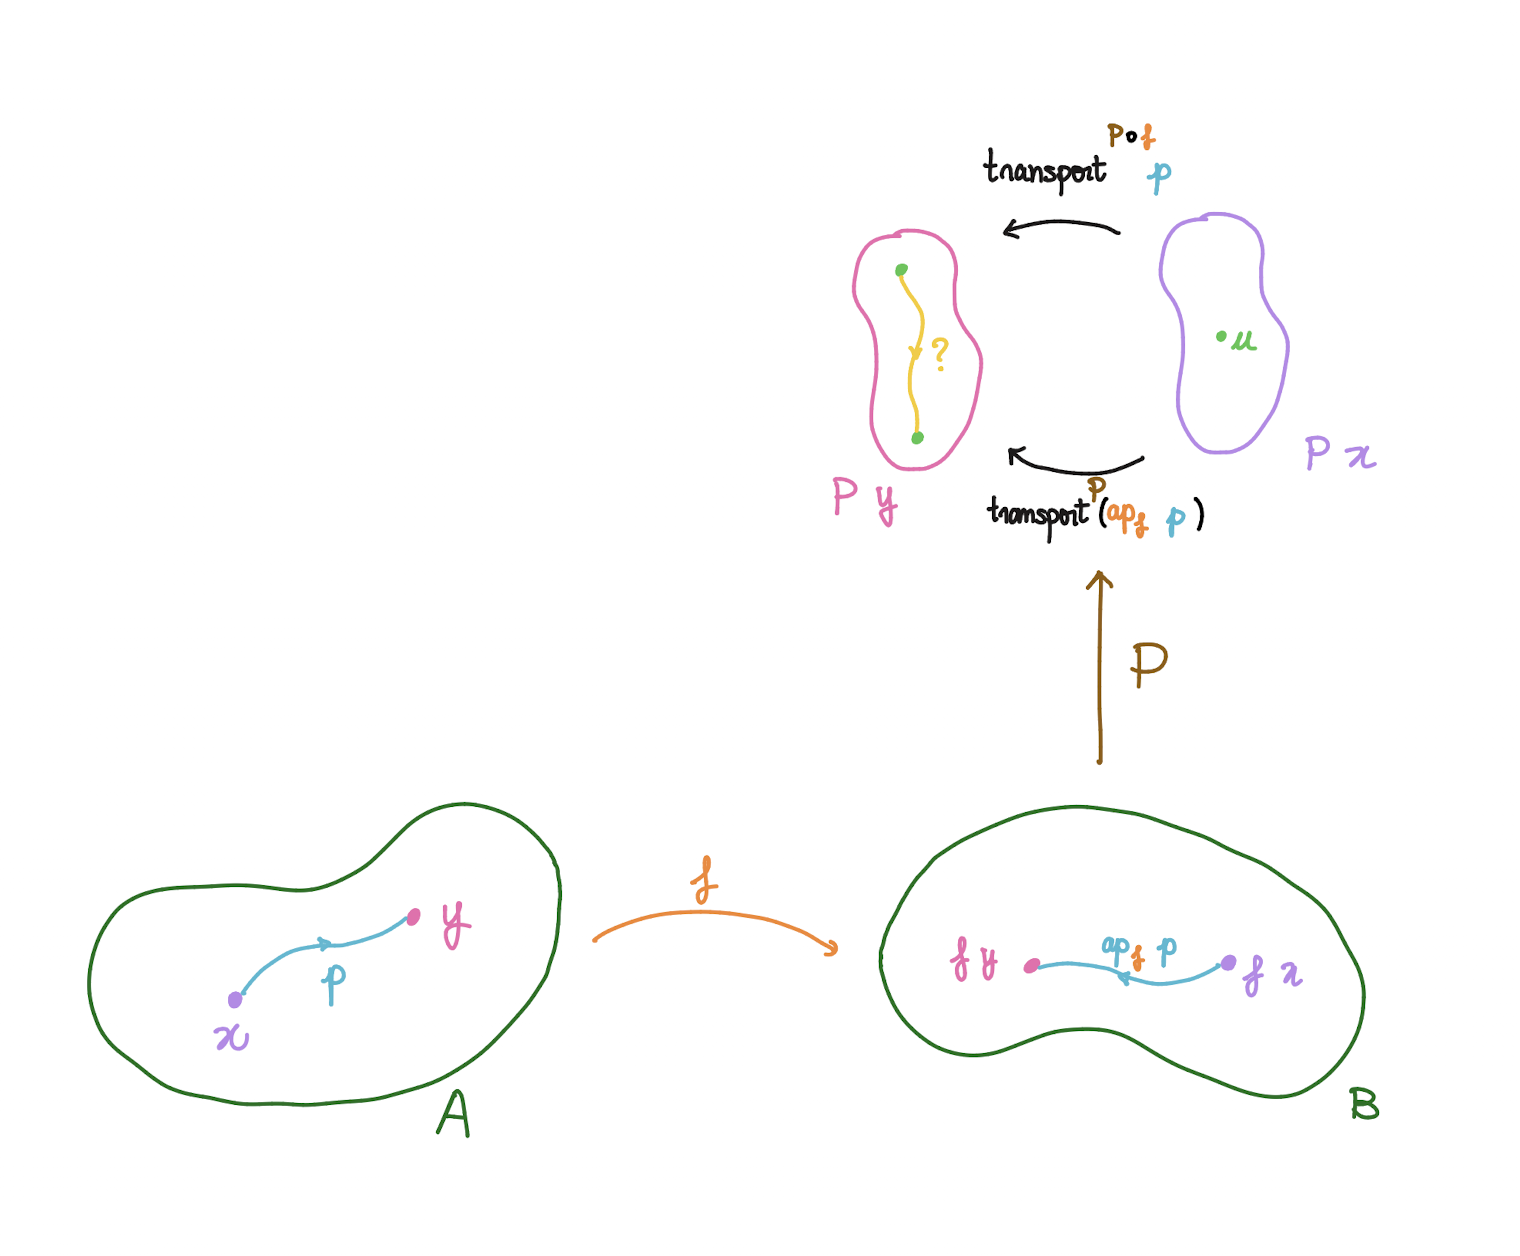
\includegraphics[width=0.8\textwidth]{transport_postcompose.png}
\caption{visualization of $\transportpostcompose$}
\end{figure}

\begin{lstlisting}
Definition transport_paths_FlFr (A B : Type) (f g : A -> B) {x y : A} (p : x = y):
forall (q : f x = g x), transport (fun z => f z = g z) p q = (ap f p)^ @ q @ (ap g p).
Proof.
    induction p.
    intro q.
    refine (_ @ (whiskerR (concat_1p q) (reflexivity (g x)))^).
    exact ((concat_p1 q)^).
Defined.
\end{lstlisting}

Note the use of the tactic \texttt{refine}. This tactic matches the goal against the co-domain of a function, in this case $\lambda p.\, p \conc (\whiskerR (\concatonep q) \refl_{g x})^{-1}$, and turns the goal into the missing argument(s) of the function, written with ``$\_$''. This effectively allows us to work backwards from the goal.

$\transportpathsFlFr$ has several special cases : for example when $B \equiv A$, $f \equiv \id_A$ and $g \equiv \lambda z. \, a$ for some $a : A$ it reduces to $\trans^{\lambda z. \, z = a} p q = p^{-1} \conc q$. We call this case $\transportpathsr$.

\begin{figure}
  \centering
    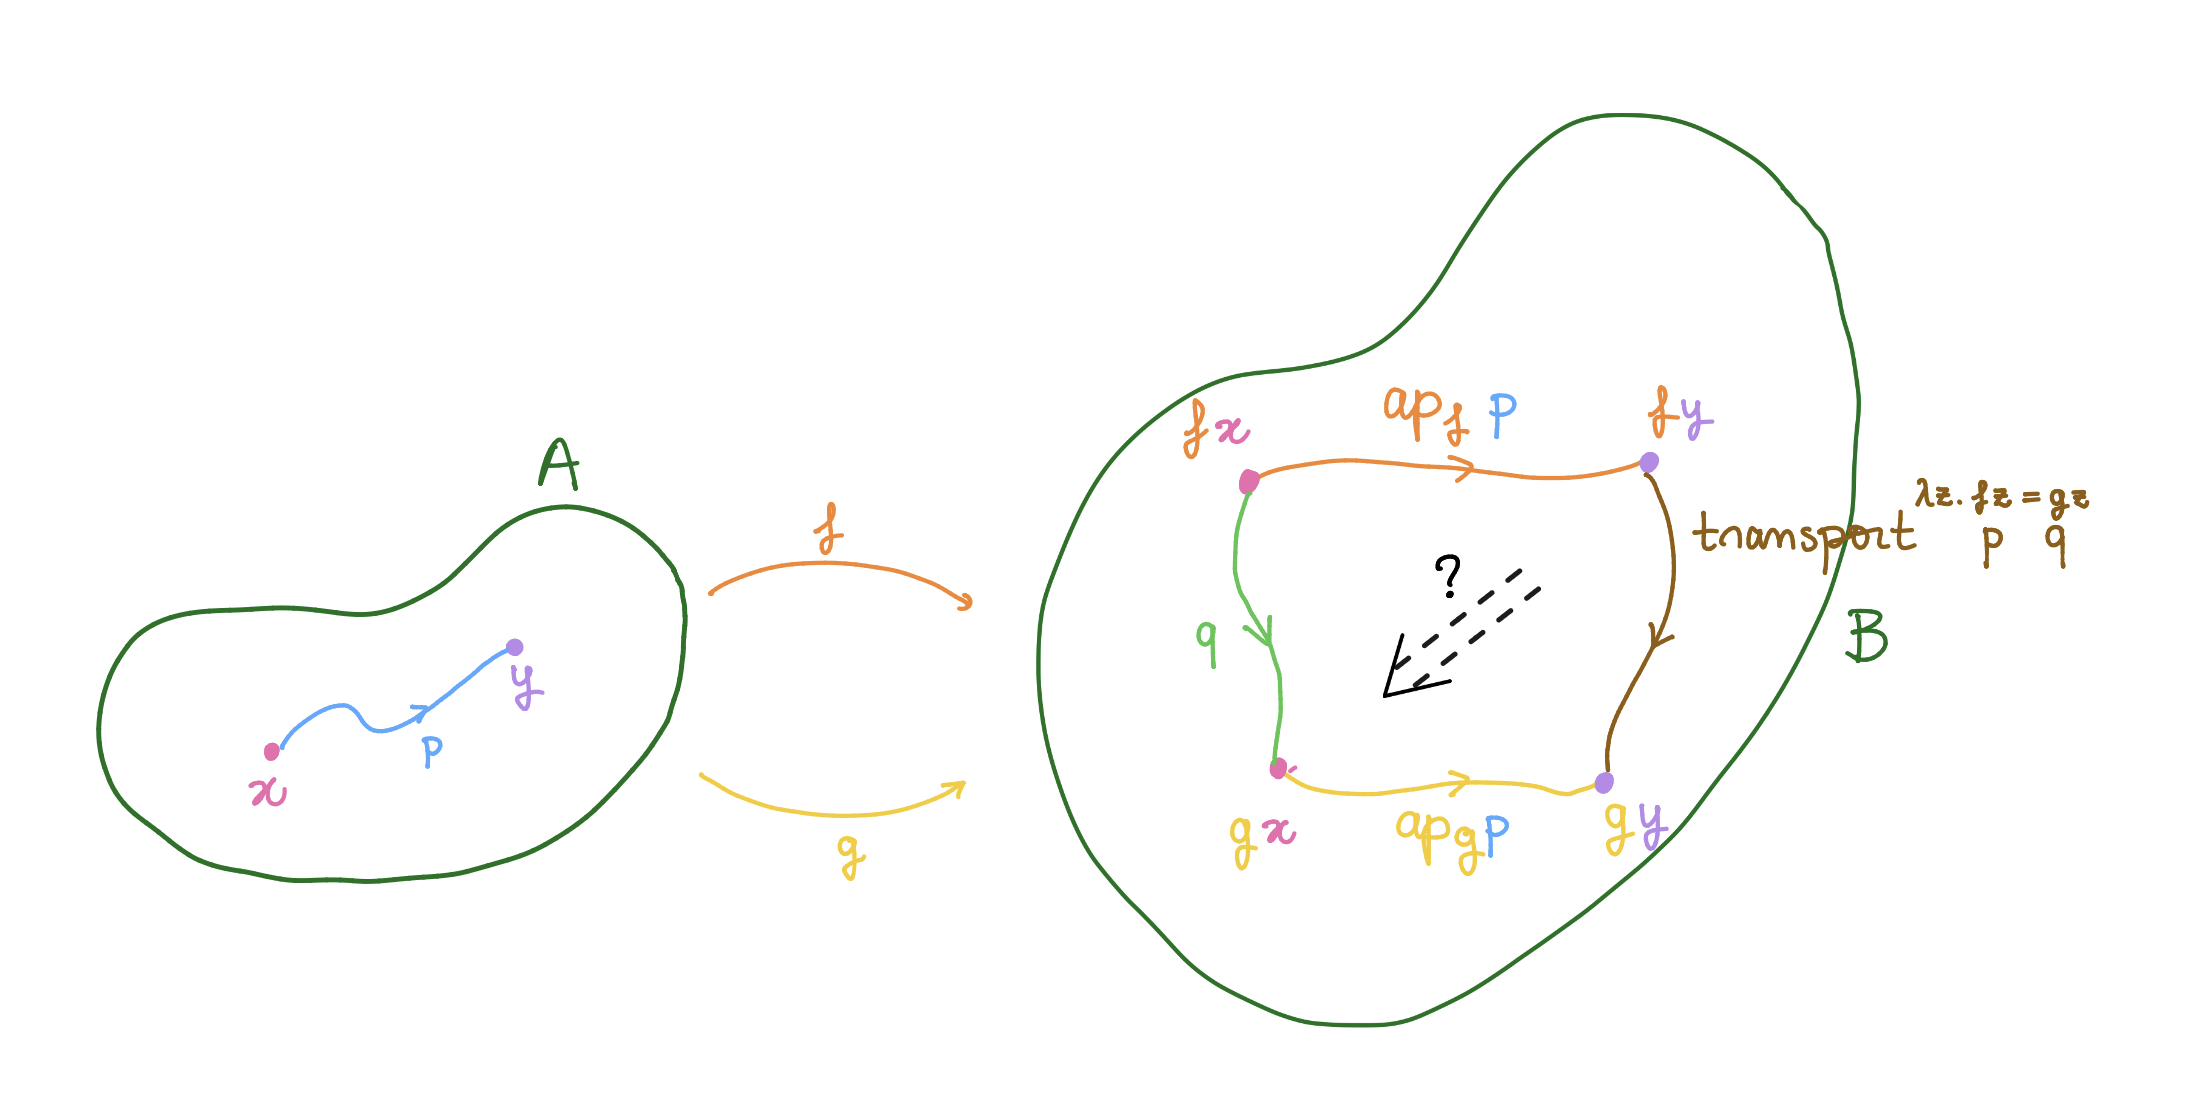
\includegraphics[width=0.8\textwidth]{transport_pathsFlFr.png}
  \caption{visualization of $\transportpathsFlFr$}
\end{figure}


\begin{lstlisting}
Definition transport_arrow {X : Type} (A B : X -> Type) {x y : X}  
(p : x = y) (f : A x -> B x):
 p # f = (fun u => transport B p (f (transport A p^ u))).
Proof.
    induction p.
    reflexivity.
Defined.
\end{lstlisting}
\begin{figure}
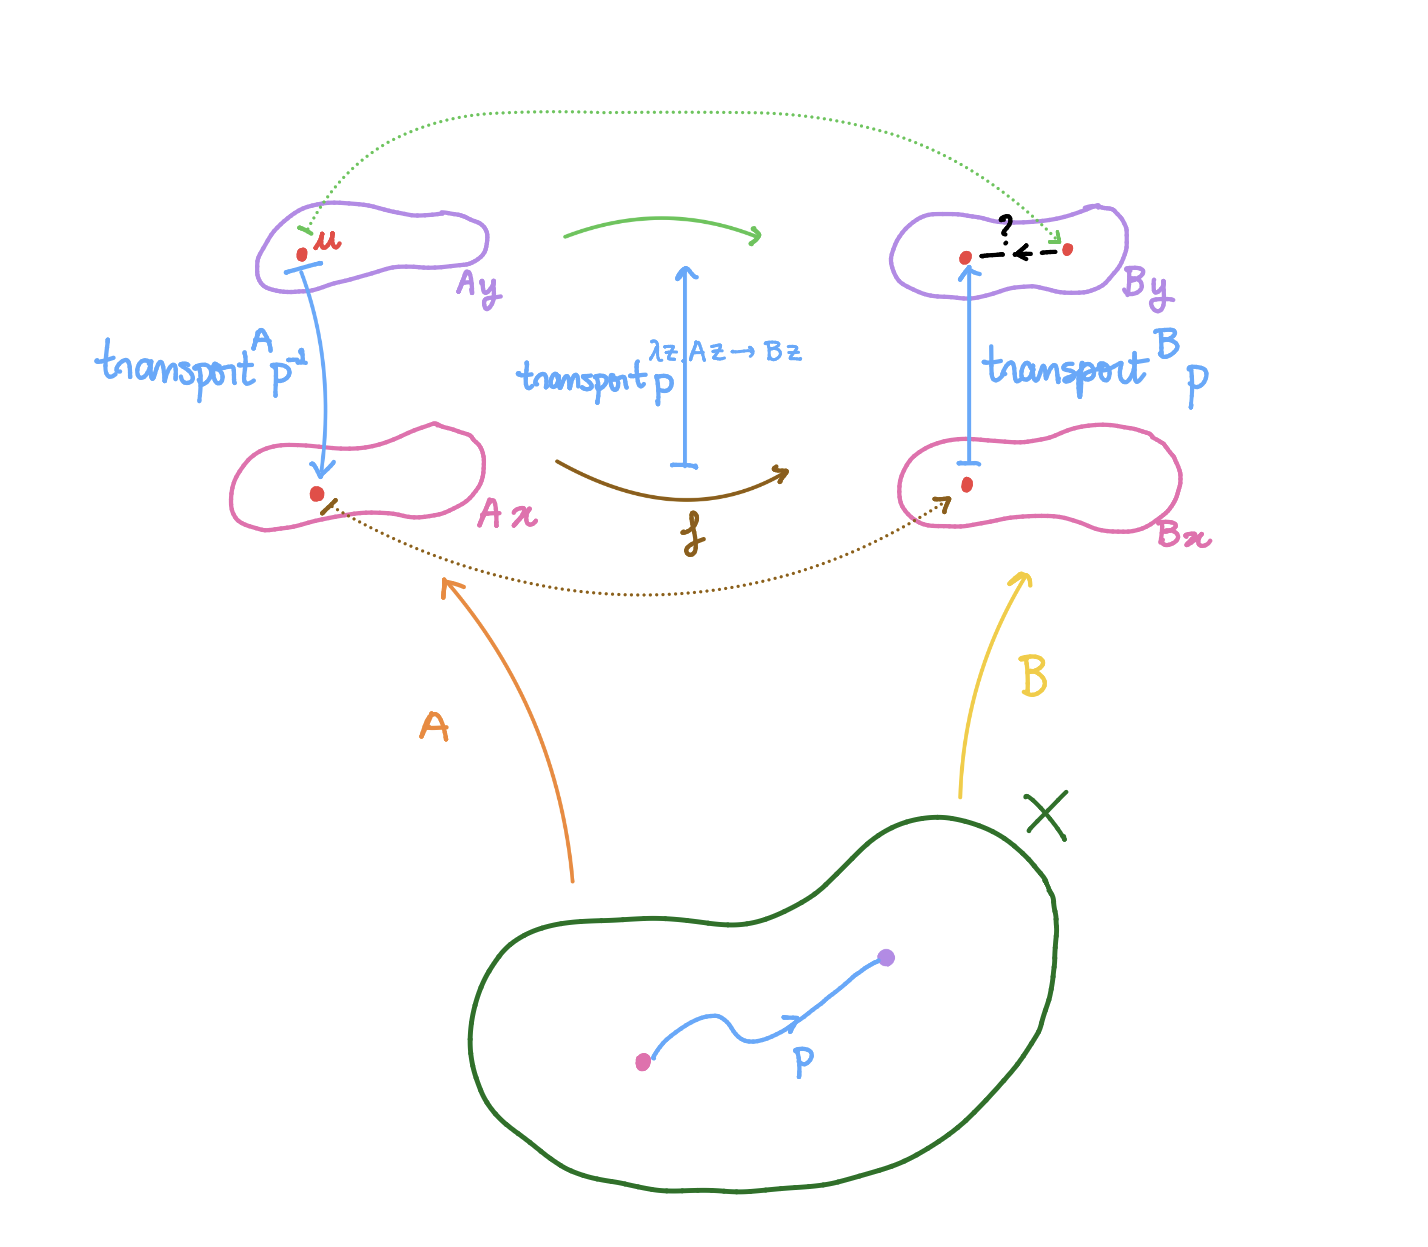
\includegraphics[width=0.8\textwidth]{transport_arrow.png}
\caption{visualization of $\transportarrow$}
\end{figure}


\section{Characterizing equality in type formers}

\subsection{Equality in Function Types}

We can easily turn equalities between (dependent) functions into homotopies in a functorial way, using the following element:

\begin{lstlisting}
Definition happly {A : Type} {P : A -> Type} (f g : forall (x : A), P x) :
f = g -> f == g.
Proof.
    intro p.
    induction p.
    exact (fun x => reflexivity (f x)).
Defined.
\end{lstlisting}

We would like to have a converse, i.e., a way to turn homotopies into equalities that makes $\happly$ an equivalence. However, there is nothing we can use to assemble a collection of paths $\prod_{x : A} f\,x = g\,x$ into a ``global'' path $f = g$. Thus, we introduce it as an axiom: the axiom of function extensionality.

\begin{axiom}
\[\funext : \prod_{A : \Type} \prod_{P : A \to \Type} \prod_{f g : \prod_{x : A} P\, x} \IsEquiv\, (\happly\, f\, g)\]
\end{axiom}

From this we can extract a function $f \sim g \to f = g$. This function is implemented in the Coq-HoTT library as \texttt{path\_arrow}.

We can also extract the homotopies between the two compositions and respective identities, and from these conclude that the operations on paths between functions are performed point-wise \cite[Section 2.9]{hottbook}.


\subsection{Equality in Universes}

Just as an equality between functions gives rise to a homotopy, an equality between types induces an equivalence. If we have a path $p : A \simeq B$, then we can extract functions $f : A \to B$ and $g : B \to A$ by transporting along $p$ and $p^{-1}$, over the type family $\id_\Type$. 
These are quasi-inverses, as stated in subsection \ref{subsec:trans}. Formally, we have: 

\begin{lstlisting}
Definition equiv_path {A B : Type}:
A = B -> A <~> B.
Proof.
    intro p.
    refine (Build_Equiv A B (transport idmap p) _).
    refine (isequiv_adjointify (transport idmap p) (transport idmap p^) _ _).
    * induction p.
      reflexivity.
    * induction p.
      reflexivity.
Defined.
\end{lstlisting}


As was the case for function types, to provide a converse we need to introduce an extra axiom: the univalence axiom.

\begin{axiom}
\[\ua : \prod_{A B : \Type} \IsEquiv \,( \idtoeqv\,A\,B)\]
\end{axiom}

The function associated to this equivalence is written in the library as \texttt{path\_universe}. The homotopies in this equivalence can be written as:

\begin{itemize}
\item$\_ : \trans^{\id_\Type} \, (\ua\, f) \sim f$
\item $\_ : \prod_{p : A = B} \ua (\trans^{\id_\Type}\, p) = p$
\end{itemize}

The first one acts as a propositional computation rule for the univalence axiom, and is written \texttt{transport\_idmap\_path\_universe} in the library, while the second acts as a propositional uniqueness principle.



\subsection{Equality in Coproducts}
\label{subsec:eqcoprod}

We choose to characterize equality in co-product types for two reasons. First, this will allow us to prove our first \textit{negative result}: that $\inl a \neq \inr b$ \footnote{$x \neq y$ is notation for $x = y \to \zero$}, which an essential step to show that univalence introduces non-trivial paths. The second reason is that this proof is a good introduction to the \textit{encode-decode method} -- a typical tool in Homotopy Type Theory -- which we will adopt to calculate the fundamental group of the circle. 

Our aim is to prove the following theorem.

\begin{theorem}
Let $A, B : \Type$, $a_0, a_1 : A$ and $b_0, b_1 : B$. Then:
\begin{itemize}
\item $\inl a_0 =_{A+B} \inl a_1 \simeq a_0 =_A a_1$
\item $\inl a_0 =_{A+B} \inr b_0 \simeq \zero$
\item $\inr b_0 =_{A+B} \inr b_1 \simeq b_0 =_B b_1$
\item $\inr b_0 =_{A+B} \inl a_0 \simeq \zero$
\end{itemize}
\end{theorem}

We will focus on the former two items, since the latter two are analogous to these. We are proving something about equality, so we would like to use path induction. However, it is not possible to do so when, as in this case, both ends of the equality are fixed. The encode-decode method consists of letting one of the endpoints of the path we are interested vary, and proving something \textit{more general} than we want, but that is \textit{easier to prove}, since we unlock the power of path induction.

With that in mind, we will define the type family $\code$ by coproduct induction, in the following way.

\begin{lstlisting}
Definition code 
{A B : Type} (a0: A) : A + B -> Type.
Proof.
  intro x.
  induction x as [a | b].
  * exact (a0 = a).
  * exact Empty.
Defined.
\end{lstlisting}

, i.e., $\code a_0\, (\inl a) :\equiv (a0 = a)$, while $\code a_0\, (\inl b) :\equiv \zero$. In other words, $\code a_0\, x$ is exactly what we \textit{want} the type $a_0 =_{A + B} x$ to be. Our goal is to prove the statement

\begin{equation}
\prod_{x : A + B} \prod_{a_0 : A} \prod_{x : A + B} (a_0 =_{A + B} x) \simeq (\code a_0 \, x)
\label{eq_coprod}
\end{equation} 

We will construct quasi-inverses. From left to right, we need a way to produce an element of $\code a_0 \, x$ from $p : a_0 = x$. Transport along $p$ over $\code a_0 : A + B \to \Type$ gives us a function $\code a0 \,a0 \to \code a0\, x$, so we just need an element of $\code a_0 \,a_0 \equiv a_0 = a_0$, which can be $\refl_{a_0}$. Thus, $\encode$, is defined as follows.

\begin{lstlisting}
Definition encode {A B : Type} (a0 : A) : forall (x : A + B), (inl B a0) = x -> code a0 x.
Proof.
    intros x p.
    exact (transport (code a0) p (reflexivity a0)).
Defined.
\end{lstlisting}

For the other direction, we want to produce a dependent function $\prod_{x : A + B} (\code x) \to (\inl a0 = x)$. We may do this by coproduct induction. When $x$ is $\inl a$, $\code a0\, x \equiv a_0 = a$, and there is an obvious element of $(a_0 = a) \to (\inl a_0 = \inl a)$, namely $ap_{\inl}$. When $x$ is $\inr b$ we have a contradiction, $\code \inr b \equiv \zero$. Thus, $\decode$ is defined as follows.

\begin{lstlisting}
Definition decode {A B : Type} (a0 : A) : 
forall (x : A + B), code a0 x -> (inl B a0) = x.
Proof.
    induction x.
    * exact (ap (fun c => inl B c)).
    * contradiction.
Defined.
\end{lstlisting}

To complete the proof, we need homotopies $\encodedecode : (\encode a0 x) \circ (\decode a0 x) \sim \id_{\code a_0 \, x}$ and $\decodeencode :     (\decode a_0\, x) \circ (\encode a_0\, x) \sim \id_{\inl a_0 = x}$ for each $a_0 : A$ and $x : A + B$. Let $p : \inl a_0 =_{A + B} x$. 

For $\decodeencode\, a_0\, x $, let $p : \inl a_0 = x $. This is where the great advantage of this method comes in: $p$ is a path in $A+B$ between the fixed $\inl a_0$ and the \textit{variable} $x$, so we may use path induction and assume $x \equiv \inl a_0$ and $p \equiv \refl_{\inl a_0}$. The goal then becomes solvable by reflexivity.

\begin{lstlisting}
Definition decode_encode {A B : Type} (a0 : A) (x : A + B):
(decode a0 x) o (encode a0 x) == idmap.
Proof.
    intro p.
    induction p.
    reflexivity.
Defined.
\end{lstlisting}


For the other homotopy, let $c : \code a_0 \,x$. We want to show that $(\encode a0\,x) (\decode a_0\,x\, c) = c$. We use induction on $x$ to split the goal into the cases $x \equiv \inl a$ and $x \equiv \inr b$. 

In the first case, $\decode a_0\,x \equiv ap_{\inl}$, so the goal becomes $\trans ^{\code a_0} \, (ap_{\inl} c) \, \refl_{a_0} = c$. We may use path induction on $c : a_0 =_A a$ to complete the goal immediately. In the second case, we have $c : \code a_0 \,\inr b \equiv 0$, a contradiction.

\begin{lstlisting}
Definition encode_decode {A B : Type} (a0 : A) (x : A + B): 
(encode a0 x) o (decode a0 x) == idmap.
Proof.
    intro c.
    induction x.
    * induction c.
      reflexivity.
    * contradiction.
Defined.
\end{lstlisting}

We now have all the ingredients necessary to give the family of equivalences in \ref{eq_coprod}. The important particular case we specifically wanted is 

\[\prod_{A ,B : \Type}\prod_{a : A}\prod _{b : B} \left(\inl a \neq \inr b\right)\]

We can supply the element $\mathsf{inl\_neq\_inr}:\equiv \lambda\, A\, B\, a\, b.\, \encode\, a \,(\inr b)$ of this type, and even more specifically $\zeroneqone:\equiv \mathsf{inl\_neq\_inr} \, \one \, \one \, \star \, \star : \boolzero \neq \boolone$.

\section {Some consequences of univalence}
\label{sec:univ}

Univalence is a powerful tool in proving negative results, i.e., of constructing functions into the empty type. One such result is the existence of a non-trivial loop. The other consequence we are going to explore exposes a ``flaw'' in the propositions-as-types correspondence.

\subsection{Sets and Propositions}
Before proving these results, it will be useful to introduce some terminology. We have used language like ``if we view this type as a proposition''. What that means is that we don't care about the particular elements of the type, just whether it is inhabited. This is particularly valid if all the elements of that type are equal, which motivates the following definition:

\begin{definition}
We say $A : \Type$ is a mere proposition if, for every $x, y : A$, $x =_A y$. We define the type family
\[ \IsProp :\equiv \lambda (A : \Type). \prod_{x, y : A} (x = y) : \Type \to \Type\], the proofs that $A$ is a mere proposition.
\end{definition}

Similarly, we can define a set as a type whose equality types are mere propositions.

\begin{definition}
We define the type family
\[ \IsSet : \lambda (A : \Type) . \prod_{x , y : A} \IsProp (x = y) : \Type \to \Type\]
\end{definition}

Examples of mere propositions are $\zero$, $\one$, $\IsProp A$, $\IsSet A$ for any type $A$ \cite[Section 3.1]{hottbook}, and $\IsEquiv f$ for any function $f$ \cite[Chapter 4]{hottbook}. It is an intuitive result that any mere proposition is either equivalent to $\one$ (if it's inhabited) or $\zero$ (if it's not). In the first case we call the proposition \textit{contractible}. Examples of sets (that are not propositions) are $\mathbb{N}$ and $\bool$ \cite[Chapter 3]{hottbook}. 

In this language, the first result we are going to prove shows that not every type is a set, while the second will show that we need to be careful when interpreting types that are not mere propositions as such. 

\subsection{A non-trivial loop}
\label{subsec:nontrivialloop}
We want to use univalence to prove a statement of the form $(p =_A \refl_x) \to \zero$. One good idea is to pick $A$ to be a type universe, $x$ to be a type and $p$ to be the result of applying the univalence axiom to some non-trivial autoequivalence. Thus, we want to choose $x$ as simple as possible, but with enough data so as to allow for a non-identity endomorphism -- the Booleans answer that description. Thus, we define $e : \bool \to \bool$ by induction as $e\, \boolzero \equiv \boolone$ and $e\, \boolone \equiv \boolzero$.

The first step is to check that $e$ is an equivalence. But $e$ is its own quasi-inverse, since $(e\circ e)\, \boolzero \equiv \boolzero$ and $(e\circ e)\, \boolone \equiv \boolone$, which, by induction, are the only cases we need to verify.

This way, we have $p :\equiv \ua\,e: \bool = \bool$. To give a function in $p = \refl_\bool \to 0$, we take an arbitrary proof of $p = \refl_\bool$, say $c$, and construct a contradiction. We will do this by repeateadly using the tactic \texttt{pose}, which creates local abbreviations for elements we define.

\begin{lstlisting}
Definition p_neq_refl : (p = reflexivity Bool) -> Empty.
Proof.
    intro c.
    pose (r1 := ap (equiv_path Bool Bool) c).
    pose (r2 := (equiv_path_path_universe E)^ @ r1).
    pose (r3 := ap equiv_fun r2).
    pose (r4 := apD10 r3 (inr tt)).
    exact (zero_neq_one r4).
Defined.
\end{lstlisting}

This proof can look quite unreadable. However, as we write it in Coq, it shows us the types of the elements we are introducing, which makes it just like writing the following on paper:

\begin{eqnarray}
    p = \refl_\bool \nonumber & \text{by hypotheses} \\
    \idtoeqv\, p = id_\bool \nonumber  & \text{by}\,\, \ap (\idtoeqv \,\bool \,\bool)  \\ 
    e = \id_\bool \nonumber  &  \text{by}\,\,(\equivpathpathuniverse \,e)^{-1} \\
     \prod_{x : \bool} (e\,x = x) & \text{by}\,\, \happly \nonumber \\
     \boolzero = \boolone \nonumber & \text{by application at} \, \boolone\\
     \zero & \text{by}\,\, \zeroneqone\nonumber
\end{eqnarray}


It is worthwhile to take a moment to think about what we've just proved. We already had a preexisting negative result, namely that $\boolzero \neq \boolone$. Using univalence, we were able to turn this result about points into a negative result about \textit{paths}: we proved that $\Type_0$, has a richer path structure that makes it not a set. In the next sections we will be able to exploit this to prove that the circle is also not set.

\subsection{Double negation}
\label{subsec:dubneg}

Another negative result we can prove using this non-trivial loop is that the law of double negation does not hold for all types. More precisely, we have the following theorem.

\begin{theorem}
We have an element of the type
\[\no \prod_{A : \Type} \left((\no \no A) \to A\right)\]
\label{thm:double_neg}
\end{theorem}

The proof is quite technical. Clearly, the thing to do is to consider $A$ to be the Booleans. However, we won't prove the stronger statement $\no ((\no \no \bool) \to \bool)$. This is because we need a dependent function $f : \prod_{A : \Type} \left((\no \no A) \to A\right)$, to which we can apply constructions like $\apd$, in order to derive a contradiction, and not just an element of $((\no \no \bool) \to \bool)$. 

The first observation that will help us prove theorem \ref{thm:double_neg} is that for any type $B$, $\no B$  is a mere proposition. This is a consequence of function extensionality.

\begin{lstlisting}
Definition neg_is_prop {A : Type} (u v : ~ A) : u = v.
Proof.
    apply (path_arrow).
    intro f.
    contradiction.
Defined.  
\end{lstlisting}

Now, this is where we can spot a difference between $\no\no \bool$ and $\bool$ : the former is a mere proposition, while the latter is not, due to $\zeroneqone$. This doesn't mean, however, that we can't find a map $\no\no\bool \to \bool$ -- indeed we can, since $\no\no\bool \simeq \one$ and a map $\one\to\bool$ is simply a choice of an element of $\bool$, of which there are two -- we just can't do it in a \textit{functorial} way, i.e., one that would extend to a map $\prod_{A : \Type} \no\no A \to A$.

To prove this, suppose we have $f : \prod_{A : \Type} \no\no A \to A$ (and write the argument $A$ in subscript). We will first prove the following intermediate statement.

\begin{lemma}
For all $u : \no\no\bool$, we have $ f_\bool\, u = e
\,(f_\bool (\trans^{\no\no} \,p^{-1}\, u))$, where $\no\no$ stands for the type family $\lambda \,X. \,\no\no X : \Type\to\Type$ and $p : \bool = \bool$ is the non-trivial path defined before.
\label{lemma_dn}
\end{lemma}

\begin{proof}
The idea is that we can combine our two main ingredients, $ f : \prod_{A : \Type} \no\no A \to A$ and $p : \bool =_\Type \bool$ using $\apd$, resulting in:
\[ \apd\, f\, p : \trans^{\lambda X. \, \no\no X \to X}\, p \, f_\bool = f_\bool \]

From here, we just apply lemmas previously derived, as well as the computation rule for univalence. The formalized proof is written below.

%The left hand side is an expression of the kind $\trans^{\lambda x. A\,x\to B\, x}\, q\, g$, so we can use $\transportarrow$, obtaining:
%\[ \transportarrow\, (\no\no\,) \id_{\Type}\, p \, f_\bool : \,\trans^{\lambda X. \, \no\no X \to X}\, p \, f_\bool = \lambda u. \trans^{\id_\Type} \,p\, (f_\bool (\trans^{\no\no} p^{-1} \,u))\]

%Concatenating the inverse of the first equality with the second, we can get an element

%\[r : f_\bool = \lambda u.\, \trans^{\id_\Type}\, p \,(f_\bool (\trans^{\no\no} p^{-1} \, u))\]

%Now, we turn this equality between functions into a homotopy, using $\happly$, and then apply the homotopy at $u$, to get 

%\[\happly\, r\, u : f_\bool \, u = \trans^{\id_\Type}\, p \,(f_\bool (\trans^{\no\no} p^{-1} \, u))\]

%This is very close to the statement of the lemma. Indeed, the propositional computation rule for the univalence axiom tells us that $\trans^{\id_\Type} (\ua \, e) = e$ (and $p \equiv \ua \, e$). If we turn this equality into a homotopy, using $\happly$, and then apply it to $f_\bool (\trans^{\no\no} p^{-1} \, u)$, we get the desired result.

%The same proof in Coq goes as follows.

\begin{lstlisting}
Definition nn := fun X => ~~X.
Definition f2_precomposed (f : forall (A : Type), (~~A) -> A) (u : ~~Bool) : f Bool u = e0 
(f Bool (transport nn p^ u)).
Proof.
    pose (q := apd f p).
    pose (r := q^ @ transport_arrow nn idmap p (f Bool)).
    pose (s := happly (transport_idmap_path_universe E) (f Bool (transport nn p^ u))).
    exact (happly r u @ s).
Defined.
\end{lstlisting}

\end{proof}

What we proved in this lemma was a homotopy between $f_\bool$, and $e \circ f_\bool$, precomposed with an endomorphism of $\no\no \bool$, namely $\trans^{\no\no}\,p^{-1}$. But as per our previous discussion $\no\no \bool$ is a mere proposition, so any endomorphism of it must be homotopic to the identity, and, by naturality, we can ignore it. Thus we obtain a homotopy

\[\prod_{u : \no\no\bool} f_\bool\, u = e \,(f_\bool \, u)\]

, which is formally proved as follows.

\begin{lstlisting}
Definition contr_hmt (f : forall (A : Type), (~~A) -> A) : f Bool == E o f Bool.
Proof.
    intro u.
    refine (f2_precomposed f u @ _).
    refine (ap (E o (f Bool)) _).
    exact (neg_is_prop (transport nn p^ u) u).
Defined.
\end{lstlisting}

This homotopy gives us a fixed point of $e$ for each element of $\no\no\bool$. In order to find a contradiction, all we need to do is prove that $e$ has no fixed points, and find an element of $\no\no\bool$. 

Proving that $e$ has no fixed points is easily done by induction on the booleans and using $\zeroneqone$ and its inverse.


\begin{lstlisting}
Definition no_fixed_points: forall (b : Bool), ~(b = E b).
Proof.
    induction b.
    * induction a.
      exact zero_neq_one.
    * induction b.
      exact (fun p => zero_neq_one p^).
Defined.
\end{lstlisting}

An element of $\no\no\bool$ is a function that maps functions in $\bool \to \zero$ to elements of $\zero$. Of these we can produce two: evaluation at $\boolzero$ and evaluation at $\boolone$. Choose $u :\equiv \lambda g. g\,\boolzero : \no\no\bool$. Thus, we have our desried result:

\begin{lstlisting}
Definition no_double_neg: ~(forall (A : Type), (~~A) -> A).
Proof.
    intro f.
    refine (no_fixed_points (f Bool _) (contr_hmt f _)).
    exact (fun g => g zero2).
Defined.
\end{lstlisting}


\section {Higher Inductive Types}
Inductive types already give our type theory a lot of expressive power, and allow for some interesting consequences of Univalence. However, we are not yet able to define some concrete non-trivial topological spaces that we'd wish to see realised: in fact, all the concrete types we've defined that don't involve universes are sets, and as such have no interesting topological properties like non-trivial loop spaces. 

%although induction works very well for defining a type through the elements we want it to have, it doesn't provide any way to have control over its paths.

In higher inductive types, we allow not only point (i.e.,zero-dimensional) constructors, but also for path constructors of any dimension. The induction principles require us to specify the images of functions on paths, and will give us propositional $\beta$-conversion rules for these, which will have to be introduced as extra axioms for every type we define.

There are many constructions that are made possible, such as co-equalizers of functions (and hence all co-limits), set quotients, CW-complexes, etc. \cite[Chapter 6]{hottbook}. Here, we will focus on the two simplest, which already demonstrate some of the power of higher inductive types : the interval and the circle.


\subsection{The Interval}

The interval $I$ is defined as follows.

\begin{definition}
We have a higher inductive type, $I$, with the following constructors.
\begin{itemize}
\item $0_I : I$
\item $1_I : I$
\item $\seg : 0_I = 1_I$
\end{itemize}
Its induction principle is 
\[\mathsf{ind}_I : \prod_{P : I \to \Type} \prod_{b_0 : P\,0_I} \prod_{b_1 : P\, 1_I} (b_0 =^P_{\seg} b_1) \to \prod_{x : I} P\,x\]
It comes with the judgemental computation rules
\begin{itemize}
\item $\mathsf{ind}_I\, P \, b_0 \, b_1 \, s \, 0_I\equiv b_0$
\item $\mathsf{ind}_I\, P \, b_0 \, b_1 \, s \, 1_I\equiv b_1$
\end{itemize}
Along with the axiom
\begin{itemize}
\item $\_ :\apd_{\mathsf{ind}_I\, P \, b_0 \, b_1 \, s} \, = s $
\end{itemize}
\end{definition}

From this induction principle, we can derive a non-dependent version (i.e., a \textit{recursion} principle) by choosing $P$ to be a constant type family $\lambda x. \, C$ and applying the propositional ``computation rule''  $transport\_const\,C \, \seg\, b_0 :  \trans^{\lambda x. C}\, \seg \,b_0 = b_0$, to get 

\[\mathsf{rec}_I : \prod_{C : \Type} \prod_{b_0 : C} \prod_{b_1 : C} (b_0 = b_1) \to (I \to C) \]

In Coq, we would write 
\begin{lstlisting}
Definition rec_I {C : Type} {b0 b1 : C} (s : (b0 = b1)) : interval -> C.
Proof.
    refine (interval_ind (fun (x : interval) => C) b0 b1 _).
    exact ((transport_const seg b1) @ s).
Defined.
\end{lstlisting}

%The first line applies the induction principle to the goal, i.e., it changes the goal from $I \to C$ to $\trans^{\lambda x. C}\, \seg \,b_0 = b_0$. We would like to provide $s$, but it has type $b_0 = b_1$, which is not judgementally the same as our goal. However, it is the same propositionally, since we have the element $\transconst\,C\, \lo\, b_0 : \trans^{\lambda x. C}\, \seg \,b0 = b0$. Thus, the definition is complete if we provide $(\transconst\,C\, \seg\, b0) \conc s$. 

This means that to define a function from the interval to a type $C$ we only need to provide two endpoints in $C$ and a path between those endpoints. Naturally, we want write computation rules for this recursion principle. These can be obtained from the computation rules of $\mathsf{ind}_I$. 

For the point-level rule, we have 
\[\mathsf{rec}_I \, C\, b_0\, b_1\, s\, 0_I \equiv {ind}_I \, C\, b_0\,b_1\, \,\left((\transconst\,C\, \seg\, b_0) \conc s\right) \, 0_I \equiv b_0\]. The computation rule for the image of $1_I$ is totally analogous. These are $\beta$-conversion rules just like the ones for any ordinary inductive type, and are purely judgemental.

We would like to have a similar $\beta$-conversion rule on the path level, that tells us that  $\ap_{\mathsf{rec}_I \, C\, b_0\, b_1 \, s} \,\seg)$ is equal to $s$. We can achieve that only propositionally.

\begin{lstlisting}
Definition interval_rec_beta_seg {C : Type} {b0 b1 : C} (s : b0 = b1) : ap (interval_rec' s) seg = s.
Proof.
    pose (p := interval_ind_beta_seg (fun _ => C) b0 b1 (transport_const seg b0 @ s)).
    pose (q := apD_const (interval_rec' s) seg).
    exact (cancelL (transport_const seg b0) (ap (interval_rec' s) seg) s (q^ @ p)).
Defined.
\end{lstlisting}

We want to prove $\ap\, (rec_I \,C\, b_0\,b_1 \,s) \, \seg = s$. What the induction principle gives us is 
\[\apd \, (rec_I \,C\, b_0\,b_1 \,s)\, \seg = \transconst\, C\, \seg, b_0 \conc s\]
But $\apd \, (rec_I \,C\, b_0\,b_1 \,s)\, \seg$ is related to $\ap\, (rec_I \,C\, b_0\,b_1 \,s) \, \seg$, through $\apdconst \,(rec_I \,C\, b_0\,b_1 \,s)\, \seg$, which has type
\[\apd \, (rec_I \,C\, b_0\,b_1 \,s\,\seg = (\transconst \,C\,\seg\,b_0) \,\conc\, (\ap \, (rec_I \,C\, b_0\,b_1 \,s)\,\seg )
 \]
Putting these two equalities together and cancelling $(\transconst\, C\, \lo\, b)$ on both sides yeilds the desired element.

%Notice how, in traditional topology, we first define the interval, using the real numbers and a notion of distance, and then use this object to define our notion of path. In Homotopy Type Theory, there is no need for any complicated definition of real numbers or metric spaces in order to have a notion of path (indeed we defined paths simply enough as an inductive type), and from the notion of path we can recover the notion of the interval as a topological space.

\begin{theorem}
The interval is contractible with center $0_I$, i.e. $\prod_{x : I} 0 = x$ is inhabited.
\end{theorem}

\begin{proof}
\begin{lstlisting}
Definition interval_is_contractible : {b : interval & forall (x : interval), b = x}.
Proof.
    refine (exist _ zero _).
    refine (interval_ind (fun x => zero = x) (reflexivity zero) seg _).
    refine (transport_paths_r seg (reflexivity zero) @ _).
    exact (concat_1p seg)
Defined.
\end{lstlisting}

We apply interval induction. For the image of $0_I$ we can provide $\refl_{0_I}$ and for the image of $1_I$ we have $\seg$. The goal then becomes the image of $\seg$, which should be an element of type $\refl_{0_I} =^{\lambda x.\, 0_I = x}_\seg \seg$. This is achievable by instantiating the lemmas $\concatonep$ and $\transportpathsr$ from previous sections.
\end{proof}

\subsection{The Circle}
\label{subsec:circle}

\begin{definition}
We have a higher inductive type, $C$, with constructors
\begin{itemize}
\item $\base : \C$
\item $\lo : \base = \base$
\end{itemize}
, and induction principle
\[ \mathsf{ind}_{\C} :  \prod_{P : \C \to \Type} \prod_{b : P\,\base} \left((\trans^P \lo \,b) = b \right)\to \prod_
{x : \C} P\,x\]
Additionally, we have the judgemental equality
\[(\mathsf{ind}_{\C}\, P \, b \, l )\, \base \equiv b\]
, as well as the propositional equality
\[\_ : \apd \,(\mathsf{ind}_\C P \, b \, l)\; \lo = l\]
\end{definition}

Just like for the interval, we can derive the circle's recursion principle from its induction principle. 

\[\mathsf{rec}_\C : \prod_{C : \Type} \prod_{b : C} (b = b) \to (\C \to C) \]

Its computation rules are the following.

\[\mathsf{rec}_\C \, C\, b\, l\, \base  \equiv b\]

\[\_ : ap_{\mathsf{rec}_\C \, C \, b\, l\,}\, \lo = l \]

The recursion principle can be thought of as the existence part of a \textit{universal property of the circle}. The uniqueness part would correspond to saying that if two functions $f,g : \C \to A$ and  coincide on $\base$ and $\lo$ then they are the same. 

Of course, when doing Homotopy Type Theory one has to be careful about what one means by words like ``coincide'' and ``same''. Saying ``$f$ and $g$ coincide on $\base$'' means that we have $p : f\, \base = g\,\base $. But we can't translate their coinciding on $\lo$ as there being a (two-dimensional) path $q : \ap_f\,\lo = \ap_g\, \lo$, since  $\ap_f\,\lo : f \,\base = f \,\base$ and   $\ap_g\,\lo : g \,\base = g \,\base$, which are different types. However, we can express it as there being $q : \ap_f\,\lo =^{\lambda x. x = x}_p \ap_g\, \lo$. The statement ``$f$ and $g$ are the same'' means there is a homotopy between these two functions.

With that said, we can prove the following uniqueness theorem.

\begin{lstlisting}
Definition uniqueness_circle {A : Type} (f g : Circle -> A)(p :f base = g base) 
(q :transport (fun (x : A) => x = x) p (ap f loop) = (ap g loop)) : 
forall (x : Circle), f x = g x. 
Proof.
    refine (Circle_ind (fun x => f x = g x) p _).
    rewrite (transport_paths_FlFr loop p).
    rewrite (whiskerL ((ap f loop)^ @ p) (q^ @ (transport_paths_lr p (ap f loop)))).
    rewrite (concat_p_pp ((ap f loop)^ @ p) (p^ @ ap f loop) p).
    rewrite (concat_pp_p (ap f loop)^  p (p^ @ ap f loop)).
    rewrite (whiskerL (ap f loop)^ (concat_p_Vp p(ap f loop))).
    exact (whiskerR (concat_Vp (ap f loop)) p @ (concat_1p p)).
Defined.
\end{lstlisting}

%The desired homotopy is a dependent function out of the circle, so the way to define it is through circle induction. After executing the first line, the new goal becomes $p = ^{\lambda x. f\,x = g\,x}_\lo p$. To unfold this, we use lemma \ref{}, which is done in the second line. Afer that, the goals becomes $((\ap_f \,\lo)^{-1} \conc p) \conc \ap_g\,\lo = p$. Now, we can use $q$ and lemma \ref{} to replace $\ap_g\, \lo$ by $(p^{-1} \conc \ap_f\,\lo) \conc p$. This corresponds to the third line, and gives us the new goal:

%\[ ((\ap_f\,\lo)^{-1} \conc p) \conc ((p^{-1} \conc \ap_f \, \lo) \conc p) = p \]

%Proving this goal is just a matter of using associativity and cancelation laws, which is done in the remaining lines.

We can package the universal property nicely in an equivalence, as follows.

\begin{theorem}
For any $A:\Type$, we have an equivalence
\[(\C \to A) \simeq \sum_{x \in A} (x = x)\]
\end{theorem}

\begin{proof}
\begin{lstlisting}
Definition univ_prop_circle `{Funext}(A : Type): 
  (Circle -> A) <~> {x : A & x = x}.
Proof.
    pose (f := fun (h : Circle -> A) => exist (fun x => x = x) (h base) (ap h loop)).
    pose (g := sig_ind (fun _ => Circle -> A) (Circle_rec A)).
    refine (Build_Equiv (Circle -> A) {x : A & x = x} f  (isequiv_adjointify f g _ _)).
    * intro y.
        induction y as (x,p).
        refine (path_sigma(fun x => x = x) _ _ (reflexivity x) _).
        exact (Circle_rec_beta_loop A x p).
    * intro h.
        apply path_arrow.
        refine (uniqueness_circle (g (f h)) h (reflexivity (h base)) _).
        exact (Circle_rec_beta_loop A (h base) (ap h loop)).
Defined.
\end{lstlisting}
\end{proof}

At first glance, the circle looks like the unit type, only with an explicit loop. However, the circle being contractible would destroy the analogy we are making with topology. Let us then attempt to prove that the circle is contractible, and see what obstacles we find.

We want to define a function of type $\prod_{x:\C} \base = x$ (since $\base$ is the only point in the circle we have to work with). For that, we naturally used the induction principle, with $P :\equiv \lambda x. \base = x$. For the image of $\base$, we have two options, $\refl_\base$ and $\lo$.

If we choose $\refl_\base$, then we would have to provide an element of $\refl_\base =^P_\lo \refl_\base$. Unfolding this type with $\transportpathsr$, this ammounts to producing an element of $\lo^{-1}\conc \refl_\base = \refl_\base$, which we have no obvious way of doing. If we instead chose $\lo$, then we would need an element of $\lo^{-1}\conc \lo = \lo$, which we also have no way of doing.

We see that the extra requirement of the induction principle of the circle, relative to the unit type (providing the ``image'' of $\lo$) prevents us from proving the circle is contractible. In fact, univalence allows us to prove that the circle is not even a set.

\begin{theorem}
If $\lo = \refl_\base$, then every type is a set.
\end{theorem}

\begin{proof}
\begin{lstlisting}
Definition loop_eq_refl_implies_is_set_Type : 
loop = reflexivity base -> forall (A : Type), IsTrunc 0 A.
Proof.
    intros H A.
    apply istrunc_S.
    intros x y.
    apply hprop_allpath.
    induction x0.
    intro l.
    exact((ap (ap (Circle_rec l)) H)^ @ (Circle_rec_beta_loop l)).
Defined.
\end{lstlisting}
\end{proof}

This theorem means that if there are types that are not sets, the circle is one of them. But in particular the universe $\Type_0$ is not a set, as proved in subsection \ref{subsec:nontrivialloop}.

\section{Computing the Fundamental Group of the Circle}

\subsection{The Integers}
There are many ways to define the integers, $\intg$, from the natural numbers. In \cite[Section 6.10]{hottbook}, they are defined as a quotient of $\nat\times\nat$. In the HoTT library, they are defined as an inductive type with constructors $0 : \intg$, $\posS : \nat \to \intg$ and $\negS : \nat \to \intg$. Here, we won't concern ourselves with the particular definition being used (they are all equivalent and produce a suitable notion of integers). It is enough to know that the type $\intg$ has the following features:

\begin{itemize}
\item There are functions $\intsucc, \intpred, \intneg : \intg\to\intg$
\item $\intsucc$ and $\intpred$ are quasi inverses, and $\intneg$ is an autoequivalence
\item There is an element 
\begin{small}
\[\intind : \prod_ {P : \intg \to \Type}
(P\,0) \to
\left(\prod_{ n :\nat}, P \,n \to P\, (\intsucc n)\right) \to
\left(\prod_ {n : \nat}, P\, (\intneg \,n) \to P ( \intpred (\intneg \, n)\right) \to \prod_{ x : \intg} P\,x\] 
\end{small}
\cite[Lemma 6.10.12]{hottbook}, satisfying the following propositional computation rules \footnote{these elements are not in the library in this exact form. However, they are defined in the accompanying Coq file.}:
\begin{itemize}
\item $\intind\, P\, d_0\, d_p\, d_n \,0 = d0$
 \item $\intind\, P \,d_0 \,d_p\, d_n\, (\intsucc n) = d_p n (\intind\, P \,d_0\, d_p\, d_n\,  n)$
\item $\intind\, P \,d_0 \,d_p\, d_n\, (\intpred (\intneg n)) = d_n n (\intind\, P \,d_0\, d_p\, d_n\, (\intneg n))$
\end{itemize}
\end{itemize}


\subsection{The fundamental group}
The aim of this section is to prove that $\base = \base$, the loop space of the circle at the base point, is equivalent to $\mathbb{Z}$. Note that $\base = \base$ is a very natural candidate for a ``fundamental group'', since equality is defined up to two-dimensional paths.  We will use the encode-decode method, just like in subsection \ref{subsec:eqcoprod}.

To define $\code$, we use circle induction. Its value on $\base$ is what we are aiming to prove the loopspace of the circle to be, i.e., the integers. We now need to provide $\ap_\code\,\lo$, which should be a path $Int = Int$, that expresses the idea that going around the circle once corresponds to adding one in the fundamental group. A good candidate is the path that results from applying univalence to the equivalence $\suc$.

Our goal now will be to construct a family of equivalences $\prod_{x : \C} (\base = x) \simeq (code x)$. For encoding, we want to take a path $p : \base = x$ in the circle and return an element of $\code x$. Transport along $p$ over $\code$ gives us a function $\mathbb{Z} \to \code x$, so we only need to pick an element of $\mathbb{Z}$ to apply it to. If we want $\encode \lo$ to be $1$, then we need an integer $k$ such that $\trans^{\code} \lo\,k = 1$. To decide, let us see what the function $\trans^{\code}\, \lo $ does.

\begin{lemma} For any integer $k$, we have
\begin{enumerate}
    \item $\trans^{\code}\,\lo\, k = \suc\, k$
    \item $\trans^{\code}\,\lo^{-1}\, k = \pred\, k$
\end{enumerate}
\label{lemma:812}
\end{lemma}

\begin{proof}
Item $(i)$ is a matter of applying $\transportpostcompose$ and the propositional computation rules of circle induction and univalence, in the following way.

\begin{lstlisting}
Definition trans_code_loop : transport code loop == int_succ.
Proof.
    intro x.
    refine ((transport_postcompose idmap code loop x) @ _).
    pose (r := Circle_rec_beta_loop Type Int (path_universe eq_succ)).
    refine (((happly (ap (transport idmap) r))) x @ _).
    exact (happly (transport_idmap_path_universe eq_succ) x).
Defined.
\end{lstlisting}

Item $(ii)$ follows from $(i)$ if we take the inverses of both sides of the equality, using some path algebra.

\begin{lstlisting}
Definition trans_code_loop_inv : transport code loop^ == int_pred.
Proof.
    intro x.
    pose (H0 := (trans_code_loop  (transport code loop^ x))^).
    pose (H1 := ap int_pred H0).
    refine ((int_succ_pred (transport code loop^ x))^ @ H1 @ _).
    exact (ap int_pred (transport_pV code loop x)).
Defined.
\end{lstlisting}

\end{proof}

Hence, to have $\trans^{\code} \lo\,k = 1$ we should pick $k = 0$, and now $\encode$ is defined.

We can define $\decode : \prod_{x : \C} \code x \to \base = x$ through circle induction. For the image of $\base$, we need a function that maps an integer to a path in $\base = \base$. This in turn can be defined by induction on the integers, in the following way.

\begin{lstlisting}
Definition decode_base := Int_ind (fun _ => base = base) (reflexivity base) (fun n l => l @ loop) (fun n l => l @ loop^).   
\end{lstlisting}

I.e., $\decodebase\, k$ is ``$\lo^k$''. The following lemma looks almost identical to the definition, and its proof is just a matter of using the computational rules for integer induction and switching between the natural numbers and integers.

\begin{lemma} For any integer $k$, we have
\begin{enumerate}[label=\roman*)]
    \item $\decodebase\, (\suc\, k) = \decodebase\, k \conc \lo$
    \item $\decodebase\, (\pred\, k) = \decodebase\, k \conc \lo^{-1}$
\end{enumerate}
\label{lemma:incrdecr}
\end{lemma}
\begin{proof} We omit the proof here, but it can be found in the accompanying \texttt{.v} file
\end{proof}

To define $\decode$ on $\lo$, we need a path in $\decodebase = ^{\lambda y. \,\code y \to \base = y}_\lo = \decodebase\,$. We can use $\transportarrow$ to unfold the left side of this equality into $\lambda x. \,\trans^{\lambda y. base = y}\, \lo \, (\decodebase  (\trans^{\code} \lo^{-1} x))$. Then, we can use function extensionality to transform the goal from an equality of functions to a homotopy. If we introduce $k : \mathbb{Z}$, the goal then becomes:

\[ \trans^{\lambda y. \, \base = y} \, \lo (\decodebase (\trans^{\code}\, \lo^{-1} k)) = \decodebase \, k \]

Which by $\transportpathsr$ is

\[\decodebase \,(\trans^{\code}\, \lo^{-1} k) \conc \lo = \decodebase \, k\]

But now we have by lemma \ref{lemma:812} that $\trans^{\code}\, \lo^{-1} k = \pred k$, so the goal becomes simply 

\[\decodebase \, (\pred\, k) \conc \lo = \decodebase\, k\]

Which after a simple manipulation can be turned into precisely the statement of lemma \ref{lemma:incrdecr}. Thus, $\decode$ is defined. Formally:

\begin{lstlisting}
Definition decode : forall {x : Circle}, code x -> base = x.
Proof.
    refine (Circle_ind (fun x => code x -> base = x) decode_base _).
    refine (transport_arrow code (fun x => base = x) loop(decode_base)  @ _).
    apply path_arrow.
    intro k.
    refine (transport_paths_r loop (decode_base (transport code loop^ k)) @ _).
    rewrite (trans_code_loop_inv k).
    refine (cancelR ((decode_base) k.-1%int @ loop) ((decode_base) k) loop^ _).
    refine (concat_pp_V ((decode_base) k.-1%int) loop @ _).
    exact (decode_base_pred k).
Defined.
\end{lstlisting}

Now all we need to do is to prove both compositions are homotopic to the respective identities. Just like in the case of co-products, proving that, for $x\in\C$, $(\decode \,x)\circ (\encode \,x) \sim \id_{\base = x}$ is trivial after path induction.

The other homotopy requires a little bit more work. We will define $\encodedecode : \prod_{x : \C}  (\encode\, x) \circ (\decode\,x) \sim \id_{\code\, x}$ by circle induction. For that we need a homotopy $\encodedecodebase (\encode\, \base ) \circ (\decode\, \base) \sim \id_{\code\, \base}$. Thankfully, since $\mathbb{Z}$ is a set, we won't need to supply any higher paths.

Let us then focus on $\encodedecodebase$. We can prove it by integer induction, as follows.

\begin{lstlisting}
Definition encode_decode_base : forall k : code base, encode (decode k) = k.
Proof.
    intro k.
    unfold encode.
    induction k.
    *   reflexivity.
    *   refine (ap encode (decode_base_succ n) @ _).
        refine (transport_pp code (decode_base n) loop zero @ _).
        refine (trans_code_loop (transport code (decode_base n) zero) @ _).
        exact (ap int_succ IHk).
    *   refine (ap encode (decode_base_pred (int_neg n)) @ _).
        refine (transport_pp code (decode_base (int_neg n)) loop^ zero @ _).
        refine (trans_code_loop_inv (transport code (decode_base (int_neg n)) zero) @ _).
        exact (ap int_pred IHk).
Defined.  

\end{lstlisting}

Putting all these ingredients together, we arrive at the family of equivalences:

\[\circlepaths: \prod_{x : Circle} (\base = x) \simeq (\code\, x)\]

And applying $\circlepaths$ to $\base$. we get an element of $(\base = \base) \simeq \mathbb{Z}$, which is what we wanted.

\section{Conclusion}
We have developed the basic constructions of Homotopy Type Theory and their formalization in Coq. In particular, we've been able to represent interesting topological spaces such as the circle in a synthetic, type-theoretic fashion and computed its fundamental group. Throughout this process, we have formalized proofs that are not yet in the library.
\newpage
\printbibliography

\end{document}


